\documentclass{include/thesisclass}
% Main File - Based on thesisclass.cls
% Comments are mostly in English
% ------------------------------------------------------------------------------
% Further files in folder:
%  - include/cmds.tex (for macros and additional commands)
%  - include/kitlogo.pdf (for titlepage)
%  - lit.bib (bibtex bibliography database)
%  - include/titlepage.tex (for layout of titelpage)
% ------------------------------------------------------------------------------
% Useful Supplied Packages:
% amsmath, amssymb, mathtools, bbm, upgreek, nicefrac,
% siunitx, varioref, booktabs, graphicx, tikz, multicol





%% -------------------------
%% |    Thesis Settings    |
%% -------------------------
% english or ngerman (new german für neue deutsche Rechtschreibung statt german)
\SelectLanguage{english}
% details on this thesis
\newcommand{\thesisauthor}{Chenran Xu}
\newcommand{\thesistopic}{Untersuchung der Langzeitstabilität des EDELWEISS Myon-Veto-Systems}
\newcommand{\thesisentopic}{Investigation of the long term stability of the EDELWEISS muon veto system}
\newcommand{\thesislongtopic}{Very long and very detailed description of the very interesting thesis topic (only necessary for pdfsubject tag).}
\newcommand{\thesisinstitute}{Institut für Experimentelle Kernphysik}
\newcommand{\thesisreviewerone}{Prof. Dr. Guido Drexlin}
\newcommand{\thesisreviewertwo}{Dr. Klaus Eitel}
\newcommand{\thesisadvisorone}{} % to use: enter names and uncomment in titlepg
\newcommand{\thesisadvisortwo}{}
\newcommand{\thesistimestart}{01.04.2015} % on titlepage
\newcommand{\thesistimeend}{30.09.2015} % on titlepage
\newcommand{\thesistimehandin}{30.10.2017} % on second page 'preamble'
\newcommand{\thesispagehead}{Bachelor Thesis: \thesisentopic} % page heading





%% ---------------------
%% |    PDF - Setup    |
%% ---------------------
% This information will appear embed into the PDF file as meta data, but will
% not be printed anywhere
\hypersetup
{
    pdfauthor={\thesisauthor},
    pdftitle={Bachelorarbeit: \thesistopic},
    pdfsubject={\thesislongtopic},
    pdfkeywords={kit,physik,bachelor,thesis,\thesisauthor}
}





%% --------------------------------------
%% |    Settings for Word Separation    |
%% --------------------------------------
% Help for separation:
% In German package the following hints are additionally available:
% "- = Additional separation
% "| = Suppress ligation and possible separation (e.g. Schaf"|fell)
% "~ = Hyphenation without separation (e.g. bergauf und "~ab)
% "= = Hyphenation with separation before and after
% "" = Separation without a hyphenation (e.g. und/""oder)

% Describe separation hints here:
\hyphenation
{
    über-nom-me-nen an-ge-ge-be-nen
    %Pro-to-koll-in-stan-zen
    %Ma-na-ge-ment  Netz-werk-ele-men-ten
    %Netz-werk Netz-werk-re-ser-vie-rung
    %Netz-werk-adap-ter Fein-ju-stier-ung
    %Da-ten-strom-spe-zi-fi-ka-tion Pa-ket-rumpf
    %Kon-troll-in-stanz
}





%% -----------------------
%% |    Main Document    |
%% -----------------------
\usepackage{lipsum} % for Lorem Ipsum text example
\usepackage{subcaption}
\usepackage{multirow,longtable}
%\usepackage[notoc,notlof,notlot]{tocbibind}
\newcommand{\mvs}{muon-veto system}

\begin{document}
    % Titlepage and ToC
    \FrontMatter

    % coordinates for background border
\newcommand{\diameter}{20}
\newcommand{\xone}{-15}
\newcommand{\xtwo}{160}
\newcommand{\yone}{15}
\newcommand{\ytwo}{-253}




\begin{titlepage}
    % background border
    \begin{tikzpicture}[overlay]
    \draw[color=gray]
            (\xone mm, \yone mm)
      -- (\xtwo mm, \yone mm)
    arc (90:0:\diameter pt)
      -- (\xtwo mm + \diameter pt , \ytwo mm)
        -- (\xone mm + \diameter pt , \ytwo mm)
    arc (270:180:\diameter pt)
        -- (\xone mm, \yone mm);
    \end{tikzpicture}



    % KIT image and sign for faculty of physics
    \begin{textblock}{10}[0,0](4.5,2.5)
        
\includegraphics[width=.25\textwidth]{include/kitlogo.pdf}
    \end{textblock}
    \changefont{phv}{m}{n}    % helvetica
    \begin{textblock}{10}[0,0](5.5,2.2)
        \begin{flushright}
            \Large FAKULTÄT FÜR PHYSIK\\\thesisinstitute
        \end{flushright}
    \end{textblock}



    % horizontal line
    \begin{textblock}{10}[0,0](4.2,3.1)
        \begin{tikzpicture}[overlay]
        \draw[color=gray]
                (\xone mm + 5 mm, -12 mm)
          -- (\xtwo mm + \diameter pt - 5 mm, -12 mm);
        \end{tikzpicture}
    \end{textblock}



    % begin of text part
    \changefont{phv}{m}{n}    % helvetica
    \centering



    % thesis topic (en and ge)
    \vspace*{3cm}
    \Huge\thesistopic\\
    \huge(\thesisentopic)\\



    % author name and institute
    \vspace*{2cm}
    \Large Bachelorarbeit\\von\\
    \vspace*{1cm}
    \huge\thesisauthor\\
    \vspace*{1cm}
    \Large am \thesisinstitute



    % possible frontimage - thanks to JabberWok
    % for publishing the img under GNU Document License
    \vspace*{1.5cm}
 	%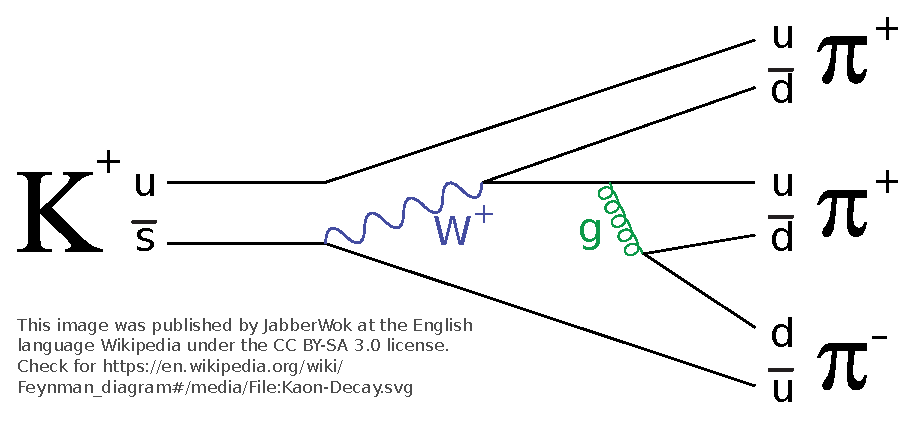
\includegraphics[scale=0.7]{./include/frontimage.eps}
 	


    % examiners (Referenten)
    \vspace*{1.5cm}
    \Large
    \begin{center}
        \begin{tabular}[ht]{l c l}
        \iflanguage{english}{Reviewer}{Referent}: 
            & \hfill & \thesisreviewerone\\
        \iflanguage{english}{Second Reviewer}{Korreferent}: 
            & \hfill & \thesisreviewertwo\\
        % uncomment if you want to provide info on your advisors
        %\iflanguage{english}{Advisor}{Betreuender Mitarbeiter}: 
        %    & \hfill & \thesisadvisorone\\
        %\iflanguage{english}{Second Advisor}{Zweiter betreuender Mitarbeiter}: 
        %    & \hfill & \thesisadvisortwo\\
        \end{tabular}
    \end{center}



    % working time
    \vspace{1cm}
    \begin{center}
        \large{{Bearbeitungszeit}: \thesistimestart \hspace*{0.25cm} -- %
                                   \hspace*{0.25cm} \thesistimeend}
    \end{center}



    % lowest text blocks concerning the KIT
    \begin{textblock}{10}[0,0](4,16.8)
        \tiny{KIT -- Universität des Landes Baden-Württemberg und nationales %
              Forschungszentrum in der Helmholtz-Gemeinschaft}
    \end{textblock}
    \begin{textblock}{10}[0,0](14,16.75)
        \large{\textbf{www.kit.edu}}
    \end{textblock}
\end{titlepage}

    \chapter*{Erklärung zur Selbstständigkeit}
Ich versichere, dass ich diese Arbeit selbstständig verfasst habe und keine %
anderen als die angegebenen Quellen und Hilfsmittel benutzt habe, die %
wörtlich oder inhaltlich übernommenen Stellen als solche kenntlich gemacht und %
die Satzung des KIT zur Sicherung guter wissenschaftlicher Praxis in der %
gültigen Fassung vom 17.05.2010 beachtet habe.\\

\vspace{1cm}

\renewcommand{\arraystretch}{0} % for spacing in the tabular environment

\begin{flushright}
	\begin{tabular}{rr}
		Karlsruhe, den \thesistimehandin, & \hspace*{5cm}\\[0mm]
		\cline{2-2}\\[2mm]    % the last line has height 2mm due
		& \thesisauthor       % to \arraystretch=0
	\end{tabular}
\end{flushright}

\vfill

\begin{flushright}
	Als Ansichtsexemplar genehmigt von\\
	\vspace{1cm}
	\begin{tabular}{rr}
		Karlsruhe, den \thesistimehandin, & \hspace*{5cm}\\[0mm]
		\cline{2-2}\\[2mm]    % the last line has height 2mm due
		& \thesisreviewerone  % to \arraystretch=0
	\end{tabular}
\end{flushright}

\renewcommand{\arraystretch}{1}

\cleardoublepage


    \begingroup \let\clearpage\relax    % in order to avoid listoffigures and
    \tableofcontents                    % listoftables on new pages
    %\listoffigures
    %\listoftables
    \endgroup
    \cleardoublepage



    % Contents
    \MainMatter

    \chapter{Introduction}
    \label{chap:intro}
    Astrophysical and cosmological observations over the last decades indicate the existence of some non-baryonic dark matter. By analyzing the anisotropy of the cosmic microwave background, the dark matter energy contribution to the total energy of the universe is estimated to be 27\% of the universe \cite{Pla16}. Yet, little knowledge of the particle constituent of the dark matter is obtained.

A generic class of hypothetical particles, the Weakly Interacting Massive Particle (WIMP), is a prominent candidate for the dark matter. WIMPs are often assumed to have a mass of $\mathcal{O}$(\SI{100}{GeV}), with an interaction cross section with ordinary matter of the order of the weak interaction scale.

The EDELWEISS experiment aims to search for a direct signal of elastic scattering of WIMPs on germanium nuclei. Due to the expected low rate of WIMP-nucleus scattering, the main challenge of the experiment is to understand and exclude potentially all the background events.

The detectors are surrounded by multiple layers of external shielding, which absorb and reject background radioactivity. Further backgrounds from the radioactivity of the shielding materials can be discriminated by the simultaneous readout of heat and ionization signals. The remaining neutron background causes a nuclear recoil in detectors, which can hardly be distinguished from a WIMP-signal. The neutrons are produced either by $(\upalpha,\mathrm{n})$ reaction from natural radioactivity or by cosmic-ray muons and natural radioactivity. To protect the detectors from the cosmic muon background, EDELWEISS is located in the underground laboratory in Modane (Laboratoire Souterrain de Modane, LSM), where the muon flux is reduced to 5\,$\mathrm{\mu}$/$\mathrm{m}^{2}$/d \cite{Sch13a}. The remaining muons are tagged by a \mvs{} of 46 plastic scintillator modules.

Since the start of the EDELWEISS experiment, the scintillator modules as well as the electronics have aged significantly. The goal of this work is to estimate the stability of the muon veto system over a period of several years. Four extra scintillator modules installed in 2010 are also equipped with LEDs allowing to monitor the stability of the system with this special light source.

In chapter \ref{chap:theo} the case of dark matter with focus on WIMPs is discussed, followed by a brief description of the general setup of the EDELWEISS experiment. In chapter \ref{chap:muon} the setup and the working principle of the \mvs{} is described. First, in chapter \ref{chap:ana_led} the LED events are analysed to estimate the long term stability of these four modules. Second, in chapter \ref{chap:ana_muon} the muon events are selected for the analysis of all modules. Additionally, the effective threshold of each module is determined to estimate the change of the detection efficiency of the \mvs.

    %\input{./chap/chapter1.tex}
    \chapter{Search for WIMPs with the EDELWEISS experiment}
    \label{chap:theo}
    % chapter2.tex
%motivation of the analysis of long term measurement~~ Dark Matter->WIMP->EDEILWEISS->Background

Nowadays, the search for dark matter becomes one of the central topics in astroparticle physics.  Numerous experiments aim to search for dark matter.

%enregieanteil durch CMB ,lambda-cdm,...
%outline for this chapter
%%%%%%%%%%%%%%%%%%%%%%%%%%%%%%%%%%%%%%%%%%%%%%%%%%%%%%%%%%%%%%%%%%%%%%%%%%%%%%%%
%%%%%%%%%%%%%%%%%%%%%%%%%%%%%%%%%%%%%%%%%%%%%%%%%%%%%%%%%%%%%%%%%%%%%%%%%%%%%%%%
\section{Evidences of dark matter}
In 1933, while studying on the velocity dispersion of galaxies inside the Coma galaxy cluster, F.Zwicky inferred the existence of some kind of unseen mass, which he called \textit{dunkle Materie} (dark matter). Since then, his idea was supported by numerous observations on different scales -- e.g. CMB, the Bullet Cluster.
The Bullet Cluster (1E 0657-56) consists of two clusters, which collided around $\SI{100}{Myrs}$ ago. Using gravitational lensing and X-Ray analysis, it is found that the two galaxy concentrations have moved ahead of their plasma clouds, which indicates the existence of weak-interacting dark matter.
In the following a more detailed description of evidence of dark matter in galaxy is given.
\subsection*{Galaxy rotation curve}


%%%%%%%%%%%%%%%%%%%%%%%%%%%%%%%%%%%%%%%%%%%%%%%%%%%%%%%%%%%%%%%%%%%%%%%%%%%%%%%%
%%%%%%%%%%%%%%%%%%%%%%%%%%%%%%%%%%%%%%%%%%%%%%%%%%%%%%%%%%%%%%%%%%%%%%%%%%%%%%%%
%%%%%%%%%%%%%%%%%%%%%%%%%%%%%%%%%%%%%%%%%%%%%%%%%%%%%%%%%%%%%%%%%%%%%%%%%%%%%%%%

\section{WIMP as dark matter candidate}



%%%%%%%%%%%%%%%%%%%%%%%%%%%%%%%%%%%%%%%%%%%%%%%%%%%%%%%%%%%%%%%%%%%%%%%%%%%%%%%%
%%%%%%%%%%%%%%%%%%%%%%%%%%%%%%%%%%%%%%%%%%%%%%%%%%%%%%%%%%%%%%%%%%%%%%%%%%%%%%%%
%%%%%%%%%%%%%%%%%%%%%%%%%%%%%%%%%%%%%%%%%%%%%%%%%%%%%%%%%%%%%%%%%%%%%%%%%%%%%%%%

\section{EDELWEISS-III Experiment}
  \label{edw}
  The EDELWEISS experiment is dedicated to detect the scattering of WIMP on ordinary matter at kryogenic temperature. In order to achieve the expected sensitivity down to \SI{e-9}{pb}, the main challenge is to exclude all the bacgrounds induced by radioactivity or cosmic rays. The general setup of the experiment and the possible backgrounds are summarized in section \ref{sec:edw-exp}. The remaining backgrounds can be discriminated by measurements of two channels of the signal. This working principle of Germanium Bolometers is briefly described in section \ref{edw-ge}.
  The problematic muon-induced neutrons, which cannot be distinguished from the WIMP-signal, is described in detail in chapter \ref{chap:muon}.
\subsection{Experimental setup and backgrounds at EDELWEISS}
  \label{sec:edw-exp}
  The EDELWEISS experiment is located in the underground laboratory of Mondane (\textit{Laboratoire Souterrain de Modane}, LSM). Under 1780 meters of rock, the cosmic muon flux is reduced by more than a factor \num{e6} to a reamaining rate of 5\,$\mathrm{\mu}$/$\mathrm{m}^{2}$/d, %\cite{muon-induced..}
  The remaining throughgoing muons are tagged with an active muon-vetor system, which is the outermost layer of the setup. (see fig.\ref{fig:exp-setup}). A detailed description and working principle are given in chapter \ref{chap:muon}.

  \begin{figure}[ht]
    \centering
    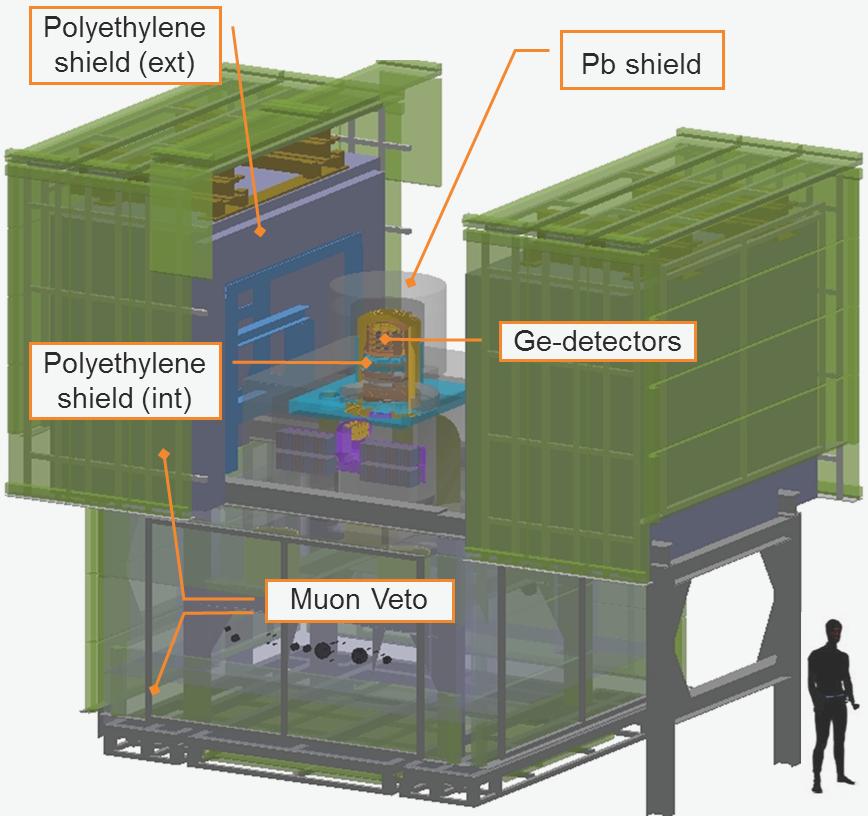
\includegraphics[width=0.75\textwidth{}]{./fig/exp_setup.png}
    \caption{\textbf{Schematic view of EDELWEISS experimental setup}.
    In the center are the Ge-bolometers hosted in a cryostat. The cryostat is surrounded by a lead shield, a PE shield and an active muon veto system to minimize the backgrounds.} Extracted from \cite{Kef16}.
    \label{fig:exp-setup}
  \end{figure}


  The next layer is a polyethylene (PE) shield of about \SI{50}{cm} thickness to attenuate the neutron flux from the radioactivity of rock and experiment materials. The fast neutron flux with energy above \SI{1}{MeV}, which produces similar recoils as from WIMPs, is reduced by 5 to 6 orders of magnitude. %\ref{backgrounds...}
  Next to the PE shield is a lead shield of 20 cm thickness to reduce the ambient $\upgamma$ background. The nature lead contains radioactive isotopes--e.g. \ce{^{210}Pb}, \ce{^{238}U} and \ce{^{232}Th}, which also contribute to the background. To reduce its natural raioactivity, the innermost \SI{2}{cm} of the shield is made of Roman lead discovered in a sunken ship. The \ce{^{210}Pb} has a half-life of $T_{1/2}=\SI{22}{years}$, so that it's abundance is decreased by two orders of magnitude. %\cite{Muon-induced background..}
  Another source of background is the \ce{^{222}Rn} as a decay product of \ce{^{238}U}. The upper part with the cryostat is installed in a clean room with renewing air to minimize the radon level. The space between the lead shield and the cryostat is flushed with filtered air.
  The upper part of the shieldings are mounted on rails and can be opened in halves to access the cryostat and electronics. Additional layers of PE and lead shields are installed inside the cryostat to reduce the background induced by electronics and cables.

  The cryostat is a \ce{^{3}He}/\ce{^{4}He} dilution refrigerator made of low-radioactivity materials. The detectors are enclosed in five thermal screens and the temperaturs decreases from room temperatur over \SI{100}{K}, \SI{40}{K}, \SI{4}{K}, \SI{1}{k} to \SI{10}{mK}. In standard operations, the temperature of the detectors is tuned to $T=(18.000 \pm 0.002)\,\si{mK}$.

\subsection{Working principle of Ge Bolometer}
  \label{edw-ge}
  The bolometers used in EDELWEISS experiment are made of high-purity monocrystalline germanium. They are equipped with aluminium ring electrodes and glued with 2 Neutron Transmutaion Doped (NTD) sensor.

  The thermalized phonon signals are measured via the change of resistence of the NTD Ge sensors. The small temperature rise resulted by a energy deposit $E_{\mathrm{rec}}$ is
  \begin{equation}
      \Delta T = \frac{E_{\mathrm{rec}}}{C{T}}
  \end{equation}
  by which $C(T)$ is the total heat capacity of the germanium crystal and two NTD sensors. The temperature dependency of resistence is given by
  \begin{equation}
    R{T}=R_{0}exp\sqrt{\frac{T}{T_{0}}}
  \end{equation}
  with charakteristic constants $R_{0}=\mathcal{O}(\SI{0.1}{\ohm})$ and $T_{0}=\mathcal{O}(\SI{1}{K})$. At the operating temerature of \SI{18}{mK}, the resistence becomes a few \si{\mega\ohm}. The NTD sensors are biased with a square modulated current and the resistence change is obtained by change of the voltage.%\cite{??}

  For each event, the ionization energy $E_{\mathrm{ion}}$ is simultaneously measured. Electron-hole pairs are produced in the germanium crystal for a energy deposit over \SI{2.96}{eV}.%cite
  The created charged carriers are drifted to the biased electodes and collected.

  The discrimination between electron recoils and nuclear recoils is based on the the ionization yield $Q$, defined as the fraction of ionization energy and recoil energy:
  \begin{equation}
    Q=\frac{E_{\mathrm{ion}}}{E_{\mathrm{rec}}}
  \end{equation}
  Since the WIMPs and neutrons scatter off nuclei, the required energy to produce a pair of charge carriers is higher than which of electron recoil. The most energy deposited by nuclear recoils are directly trainsmitted to phonons, which leads to a generally smaller ionization yield than electron reocoils.

  The heat and ionization channels are calibrated with the \SI{356}{keV} line of \ce{^{133}Ba}, which induces electron recoils.%\cite{s}
  With the ionization yield of electron recoils set to 1, the neutron ionization yield is determined with a neutron calibration:%cite
  \begin{equation}
    Q_{\mathrm{n}}=0.16\cdot(E_{\mathrm{rec}}[\si{keV}])^{0.18}
  \end{equation}
  With combination of the heat and ionization measurements, the electron recoils can be distinguished from the neutron recoils. Therefore, the remaining problematic background is neutrons, respectively produced in muon-induced showers or muon-nuclear interactions.

    \chapter{Muon detection in EDELWEISS experiment}
    \label{chap:muon}
    % chapter3.tex
% muon-veto system  Muon interaction, energy deposit, setup of muon veto, working principle, available data,
Despite the rock overburden of LSM reduces the cosmic muon flux by 6 orders of magnitude, the remaining muons can produce neutrons and mimick WIMP signals WIMPs. These muons are tagged by an active veto system. The general setup and the working principle of the system is described in this chapter. The description is mainly based on the doctoral thesis of K{\'{e}}f{\'{e}}lian. \cite{Kef16}


%%%%%%%%%%%%%%%%%%%%%%%%%%%%%%%%%%%%%%%%%%%%%%%%%%%%%%%%%%%%%%%%%%%%%%%%%%%%%%%%
%%%%%%%%%%%%%%%%%%%%%%%%%%%%%%%%%%%%%%%%%%%%%%%%%%%%%%%%%%%%%%%%%%%%%%%%%%%%%%%%

\section{Setup of the Muon veto system}
\label{sec:muon-setup}

The muon-veto system is the outermost layer of shieldings and covers a surface of $\SI{100}{m^{2}}$. As shown in the fig. \ref{fig:muon-setup}, it is made of 46 plastic scintillator modules. The modules are labelled from 1 to 48. Each wall is labelled according to the orientation. The western wall is named "Nemo", which is the name of the neighbour experiment in LSM.
The muon-veto is divided in two levels, the upper level made of 30 modules locates in a clean room and host the cryostat and the detectors. The lower level has 16 modules. As described in section \ref{sec:edw-exp}, the upper level is mounted on rails and can be opened in two parts to grant access to electronics.

\begin{figure}[ht!]
  \centering
  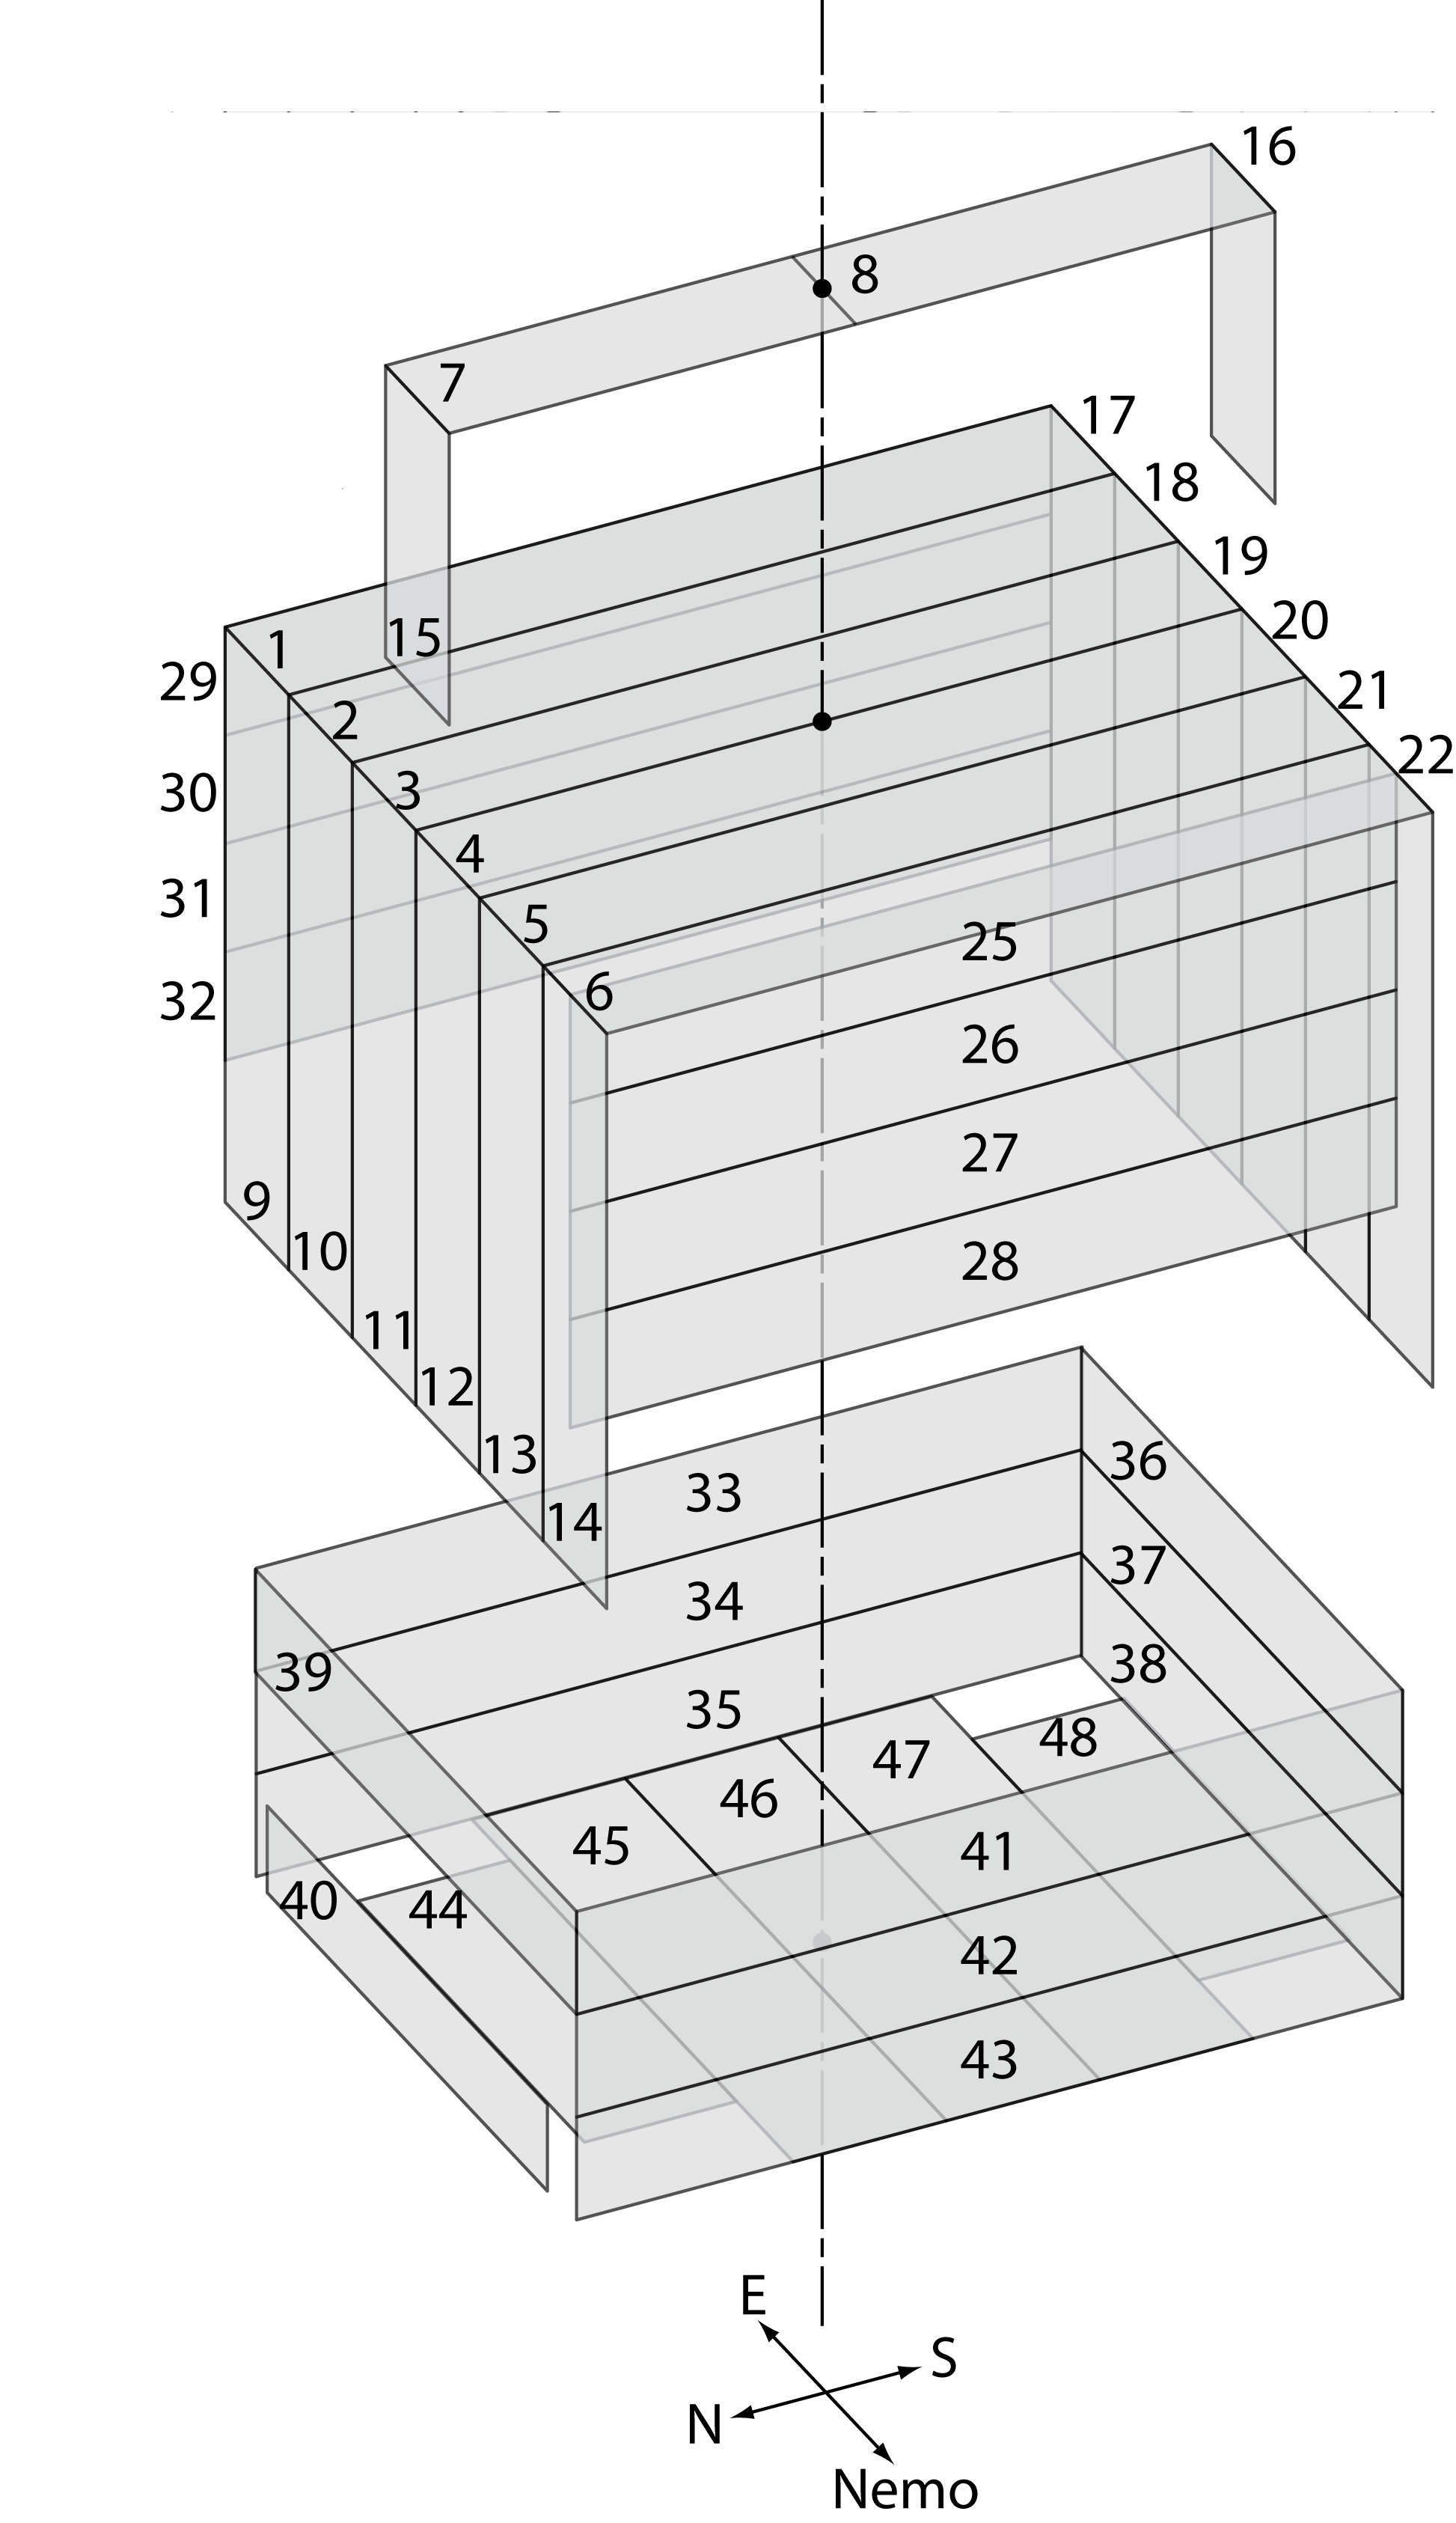
\includegraphics[width=0.5\textwidth{}]{./fig/Veto.png}
  \caption{Schematic view of Muon-Veto System. Each wall of the system is labelled according to its geometric orientation in the laboratory. }.
  \label{fig:muon-setup}
\end{figure}

To cover the gap resulted from the opening of the upper parts, M7, M8, M15 and M16 are installed in 2010. The four extra modules are equipped with LEDs to moniter the stability of the system. M7 and M8 have 3 LEDs along their axis, each of M15 and M16 has one LED installed in the middle. M7 and M8 are $\SI{2.1}{m}$ long. M15 and M16 are around $\SI{1}{m}$ long and cover only partly the opening of upper part.

The other modules have a width of $\SI{65}{cm}$ and a thickness of $\SI{5}{cm}$. Their lengths varies from $\SI{2}{m}$ to $\SI{4}{m}$.
Due to the opening for electronics and the shorter length of some modules, the overall geometric efficiency is 98\%. However, the muon going through the gap can partly be detected via the particle showers induced by them.

A group of four Photomultiplier Tubes (PMT) are installed at each module end. Each PMT group is individually biased with a high voltage (HV). The HV values are set around $\SI{-1500}{V}$ and seldom changed over years to compensate the aging effect of the modules.
To ensure the system is fully closed while operating, two lasers measure the position of two halves of the upper part every 15 minutes. One measures the distance from the western wall to M6, the other from the eastern wall to M8. The gap width is calculated by substracting the two distances.


\section{Working Principle of Muon veto system}
\label{sec:muon-working}
\end{itemize}

\subsection{Muon Energy deposit in the scintillator modules}
The average muon energy at LSM is $<E_{\upmu}>_{\mathrm{LSM}}\approx \SI{260}{GeV}$. The high energy muons deposit ~$\SI{2}{MeV\per\cm}$ in the muon-veto modules according to the Bethe formula. Since the scintillator modules have thickness of 5cm, the muon energy deposit in a module is typically above $\SI{10}{MeV}$. Therefore, the muon events can be separated from the background events with energy deposit normally lower than $\SI{4}{MeV}$, which reduces the deadtime of the experiment.
The stochastic process of muon energy deposit can be described by a Landau distribution \cite{Lan44}. Such distribution is asymmetric and has a long tail towards high energy region. To avoid the contribution of large energy deposit from the long tail, the most probable value (MPV) is usually taken to characterize the distribution.
The total energy deposit of muon is also dependent on its path length in a module. The spectrum is thus smeared due to the different orientation of modules and the angular distribution of muon flux. Most muons at LSM have small zenith angle, therefore the muons deposit minimal energy in top and bottom modules and the track length is of the order of the module thickness.
It is also possible that a muon goes through the edge of a module, which is called a \textit{grazing muon}. In such case, the muon traverses only partly the module thickness and deposits lower energy.

\subsection{Readout electronic chain}
The scintillation photons reflect in the module and are guided to the PMT groups. In a PMT group, the photons are then converted to electrons and amplified to a measurable electric signal. Once the signal amplitude is over the trigger threshold, the signal is integrated in the Analog-to-Digital-Converter (ADC) card to obtain the total energy deposit of muon in a module. At the mean time, the Time-to-Digital-Converter (TDC) card stores the time of the signal. If there is a coincidence of 2 PMT groups within $\SI{100}{ns}$ time window, all non-zero signals of the muon-veto system are stored as one event. After the triggering, there is dead-time of $\tau=\SI{0.16}{ms}$ when no events can be detected. The trigger threshold is set to $\SI{150}{mV}$ to ensure the detection efficiency of low energy events without introducing to much dead-time.

\subsection{Position-dependent light output}
In addition to the fluctuation of the muon energy deposit, the light output is also dependent on the position of the interaction in the scintillator modules. Since the light is guided up to $\SI{4}{m}$ to the PMT group, which is much larger than the attenuation length, the light measured by PMT decreases exponentially with the path length $d$. The relation can be aprroximately determined by the Beer-Lambert law:
\begin{equation}
  I(d)=I_{0}\cdot e^{-\frac{d}{\mathrm{\Lambda}_{\mathrm{eff}}}}
\end{equation}
The $\Lambda_{\mathrm{eff}}$ denotes the effective attenuation length and is a detector specific constant.
The scintillator modules in EDELWEISS were previously used in KARMEN experiment. The effective attenuation length was measured to be $\mathrm{\Lambda} \approx \SI{600}{cm}$ in 1997/1998 \cite{Rei98}. However, the modules has aged since then. Some of the effects are radiation damages and decrease of the transparency.

\begin{figure}[ht!]
  \centering
  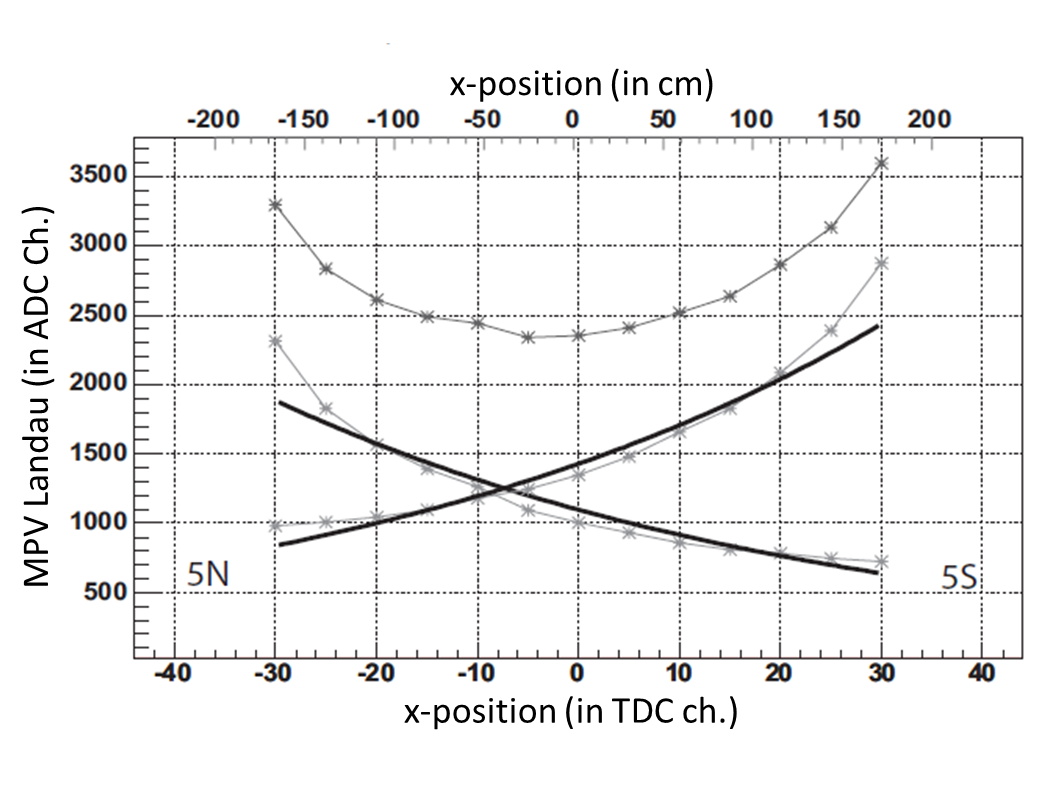
\includegraphics[width=0.6\textwidth{}]{./fig/pos-dependent.png}
  \caption{Light measured in the north and south PMT groups of Module 5 and the sum of them. The data are fitted with exponential curves. Extracted from \cite{Hab04}.}
  \label{fig:pos-dependent}
\end{figure}

In 2003/2004 the attenuation length of two $\SI{4}{m}$ modules were measured. Fig. shows the measured signal in M5 for two individual PMT groups and the sum of them. As shown in the figure, the light yield varies by a factor of 2 from the near end to far end.
For M5 $\Lambda_{\mathrm{eff}}$ was around $\SI{340}{cm}$ and for M1 around $\SI{200}{cm}$ \cite{Hab04}. The measurement shows that the effective attenuation length of scintillator modules has decreased significantly since production, which leads to a decrease of discrimination efficiency for low energy events. This also motivates the importance to analyze the long term stability of the muon-veto system.


\subsection{Available Data of the Muon-Veto Run}

The measured events are stored in data files and combined to so-called Runs. Each Run contains up to 99 files, with each file stores 8 hours measurement. The data in each Run file are converted to a KData file. KData is a ROOT-based \cite{Bru97} data structure and analysis toolkit developed at KIT. It combines the muon-veto data and the bolometer data for coincidence studies \cite{Cox12}.
The data branches relevent in the context of this work and available for the analysis are listed below:
\begin{itemize}
  \item ADC
  When triggered, the integrated signal in each PMT group is stored in ADC units. The HVs of each PMT group are calibrated before the experiment to ensure an uniform gain of each module. Since the modules have aged individually, the correspondence between ADC channels and Energy in MeV varies from module to module. There is also a conversion threshold. For an event with energy deposit under this value, the ADC is not stored and set to -1. The threshold is ~120\,ADC channels and differs from each other.

  \item TDC
  The arrive time of signal in each PMT group is stored. By substracting the two TDC values in one module, the event postion can be reconstructed. In the presented work, the TDC values are only used to probe if a PMT group is triggered.


  \item{PC Time}
  The time of each event are stored in seconds. For the muon-veto events to be compared with bolometer events, an additional timestamp in 10\,\upmu{}s precision is saved. However, such precision is of no interest in analysis of the long term stability. Therefore, the event time in seconds is used in the following analysis.

  \item{DistanceEst,DistanceNemo}
  As described before, the gap size of the upper part of the system is measured every 15 miniutes. DistanceEst stores the distance from eastern wall to M8 and DistanceNemo stores the distance from western wall to M6. For each event, the distances obtained from last laser measurement are saved.

  \item{IsLEDFired}
  The LEDs installed on extra top modules fire every eight hours to monitor the stability of the system. When the event is caused by LED firing, the bool value IsLEDFired will be set to true, allowing a distinction between LED events and other events.
\end{itemize}






%available values

    \chapter{Long term behavior of data acquired with LEDs}
    \label{chap:ana_led}
    % chapter4.tex
% LED Chapter (Muon?)
As described in Chapter \ref{chap:muon}, the four extra modules added in 2010 covering the gap of the \mvs{} are equipped with LEDs. M7 and M8 have three LEDs: one at the center and the other two symmetrically at 0.45\,m distance from the end. M15 and M16 both have one LED installed at the center. The LEDs send out pulses every eight hours. The LED data are used to perform a stability control of the \mvs{}. They are clearly defined in light emission, position and time compared to muon induced events, therefore the LED events are a good probe to estimate the long term stability of these four modules.
\section{Data selection}
For the following analyses, data of muon-veto Run70 to Run138 are used to analyse the ageing effect of the veto system. This corresponds to a date from 24.08.2010 to 28.03.2017. When converting the raw data to ROOT-format, the events induced by LED firing are flagged. Therefore, they are easily separated from other events.
The LEDs fire three times every day. Each LED fires 60 pulses in one minute and they fire one after another, which also allows a separation of signals from different LEDs in M7 and M8.

\section{HV stability}
Since the HV information is not contained in the \textit{KData} files and the HV settings are only seldom changed over the time period, the HVs are first separately investigated. For M8, M15 and M16, the HVs are not changed from year 2010 to 2017.

\begin{figure}[htb!]
  \centering
  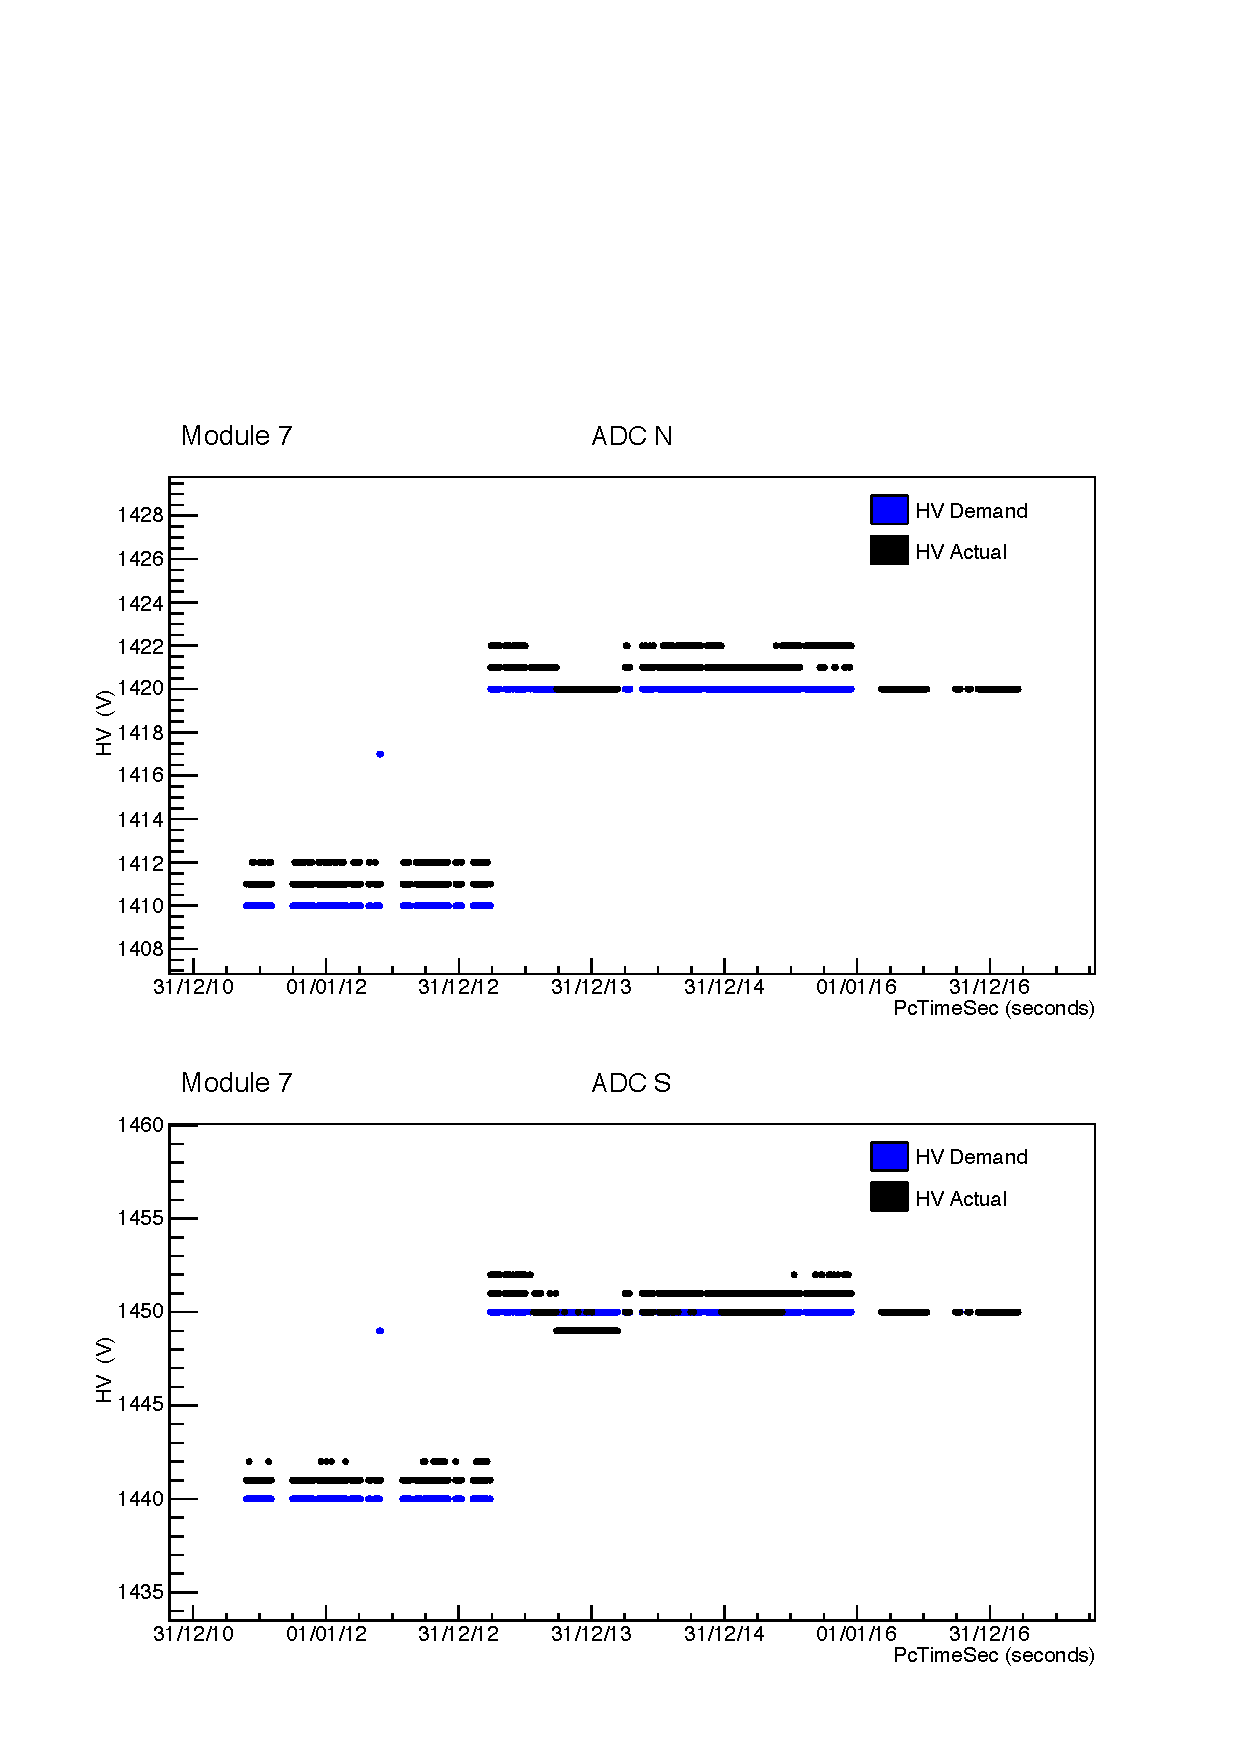
\includegraphics[width=0.8\textwidth{}]{./fig/HVPlot_M7.pdf}
  \caption{HV applied on M7 from year 2010 to 2017. The HV applied on the module is negative and the plot shows the absolute value of the HV. The blue points are the set value of the HV and the black points are the actual measured HV. In March 2013, the set HV was increased from -1410\,V to -1420\,V on the ADC N and from -1440\,V to -1450\,V on the ADC S.}
  \label{fig:HV_7}
\end{figure}

The behaviour of the HV applied on M7 is plotted in fig.\,\ref{fig:HV_7}. The plot shows the absolute value of the HV, as the HV applied on the module is actually negative. For northern PMT group, the was is increased from -1410\,V to -1420\,V in March 2013. For southern PMT group, the HV was increased from -1440\,V to -1450\,V. As seen in the figure, the measured HV values fluctuate by $\pm$3\,V from the set value.\\
For other three extra modules, the measured HV values have a fluctuation of $\pm$5\,V, which is also in the region of statistical uncertainty. The HVs are thus determined to be stable during the time period of seven years.

\section{Data Analysis}
\label{sec:led-ana}
The LEDs are fixed on the modules, so the energy spectrum is not smeared by the position dependent light readout. Also, the LEDs are supposed to have constant light output over a short time. Thus the obtained ADC spectrum can be fitted with a gaussian function to get the average ADC values of several series.
To increase the statistical power of a single point, events of nine shot series (three days) are combined to perform a gaussian fit. An example of such fit is illustrated in fig.\ref{fig:gaussian-fit}.

\begin{figure}[htb!]
  \centering
  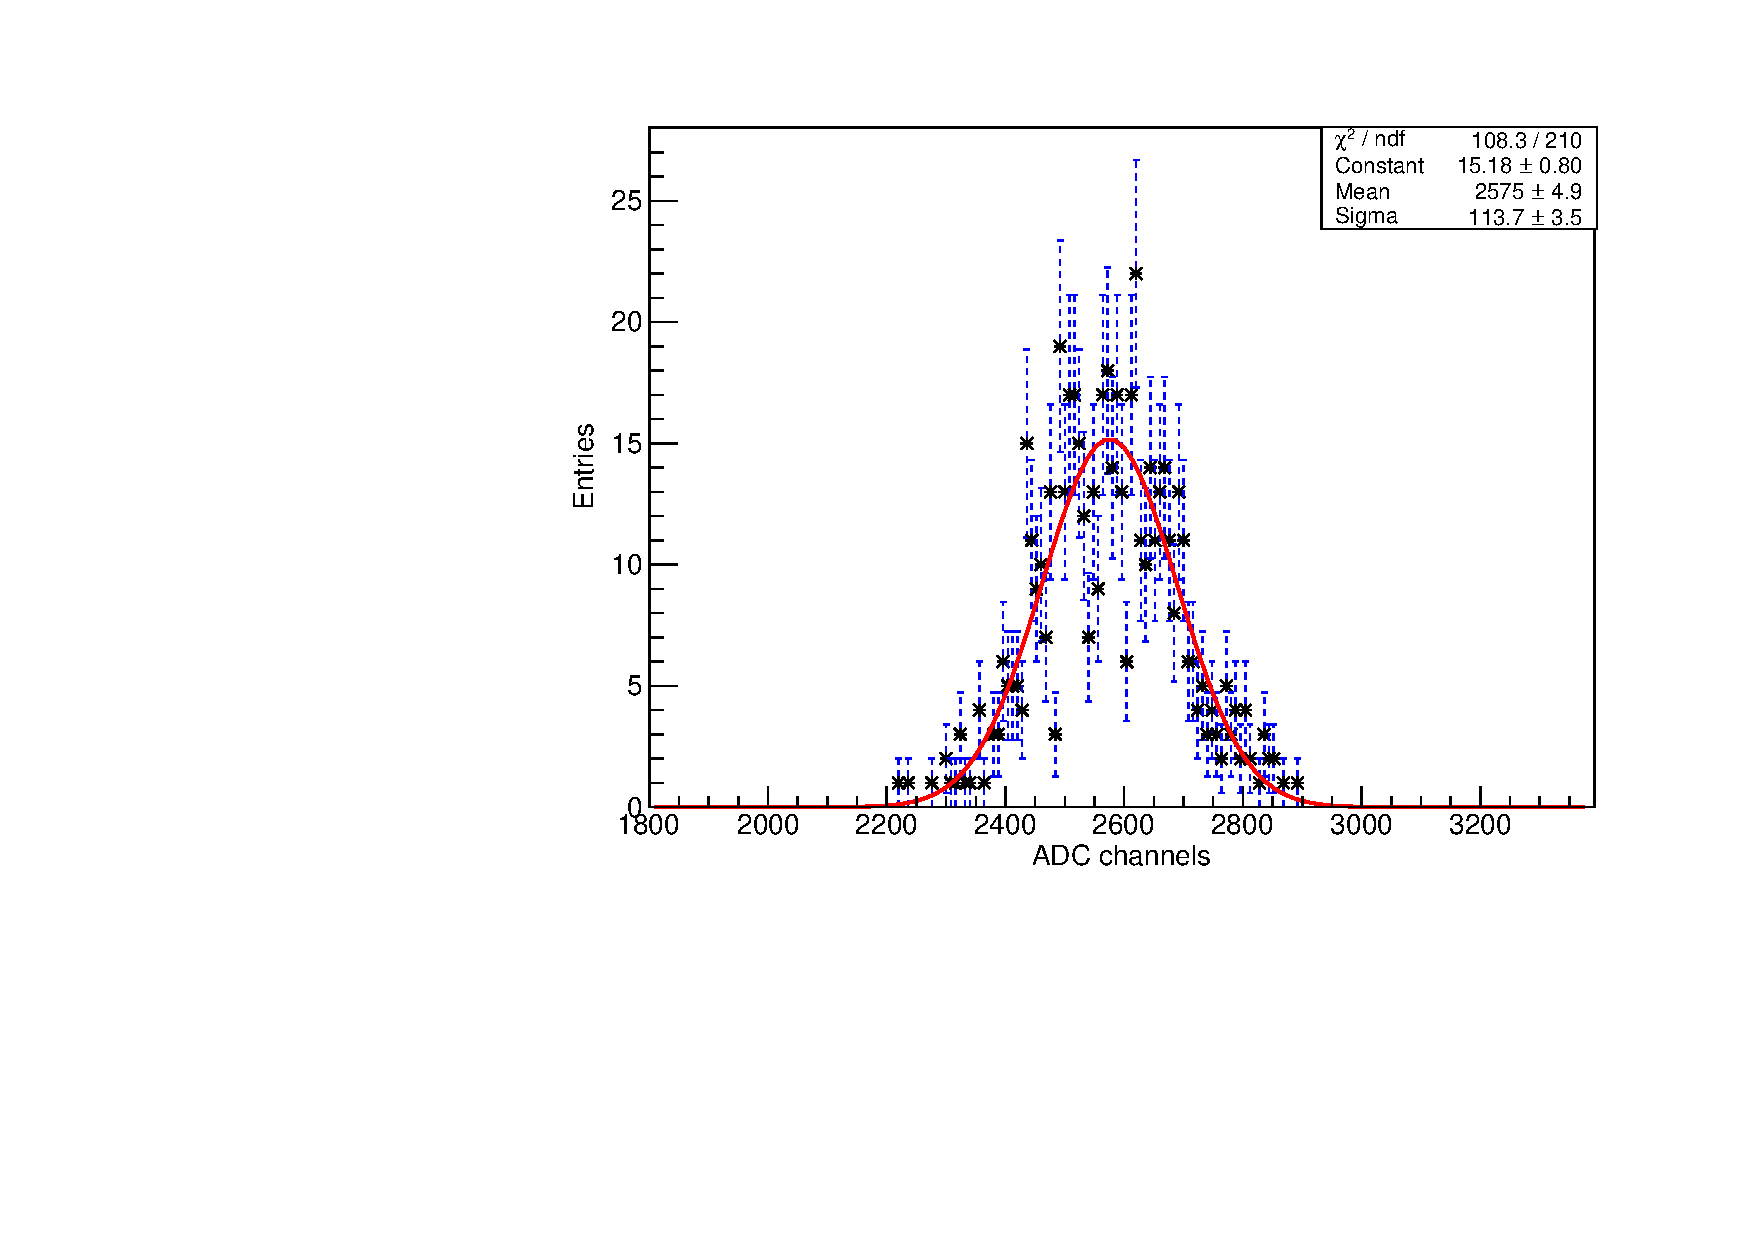
\includegraphics[width=0.8\textwidth{}]{./fig/gaussianM8.pdf}
  \caption{Example of a gaussian fit to nine LED fire series in Module 8, north PMT group. The spectrum is fitted with a log likelihood method in ROOT.}
  \label{fig:gaussian-fit}
\end{figure}

The mean ADC values obtained from each gaussian fit are plotted over time. A change of these values over time could be due to various effects, e.g.\ a decrease of the LED light output, ageing of scintillator modules, problem of the PMTs or readout electronics. To identify the contribution of different factors, the values are plotted separately for two PMT groups and three LEDs (for M7 and M8). Linear regressions are made for each data set, see fig.\ref{fig:M8LED}. The lines with different colour represent the data from different LEDs. In the following, the result is described in detail for module 8.

\begin{figure}[htbp]
  \centering
  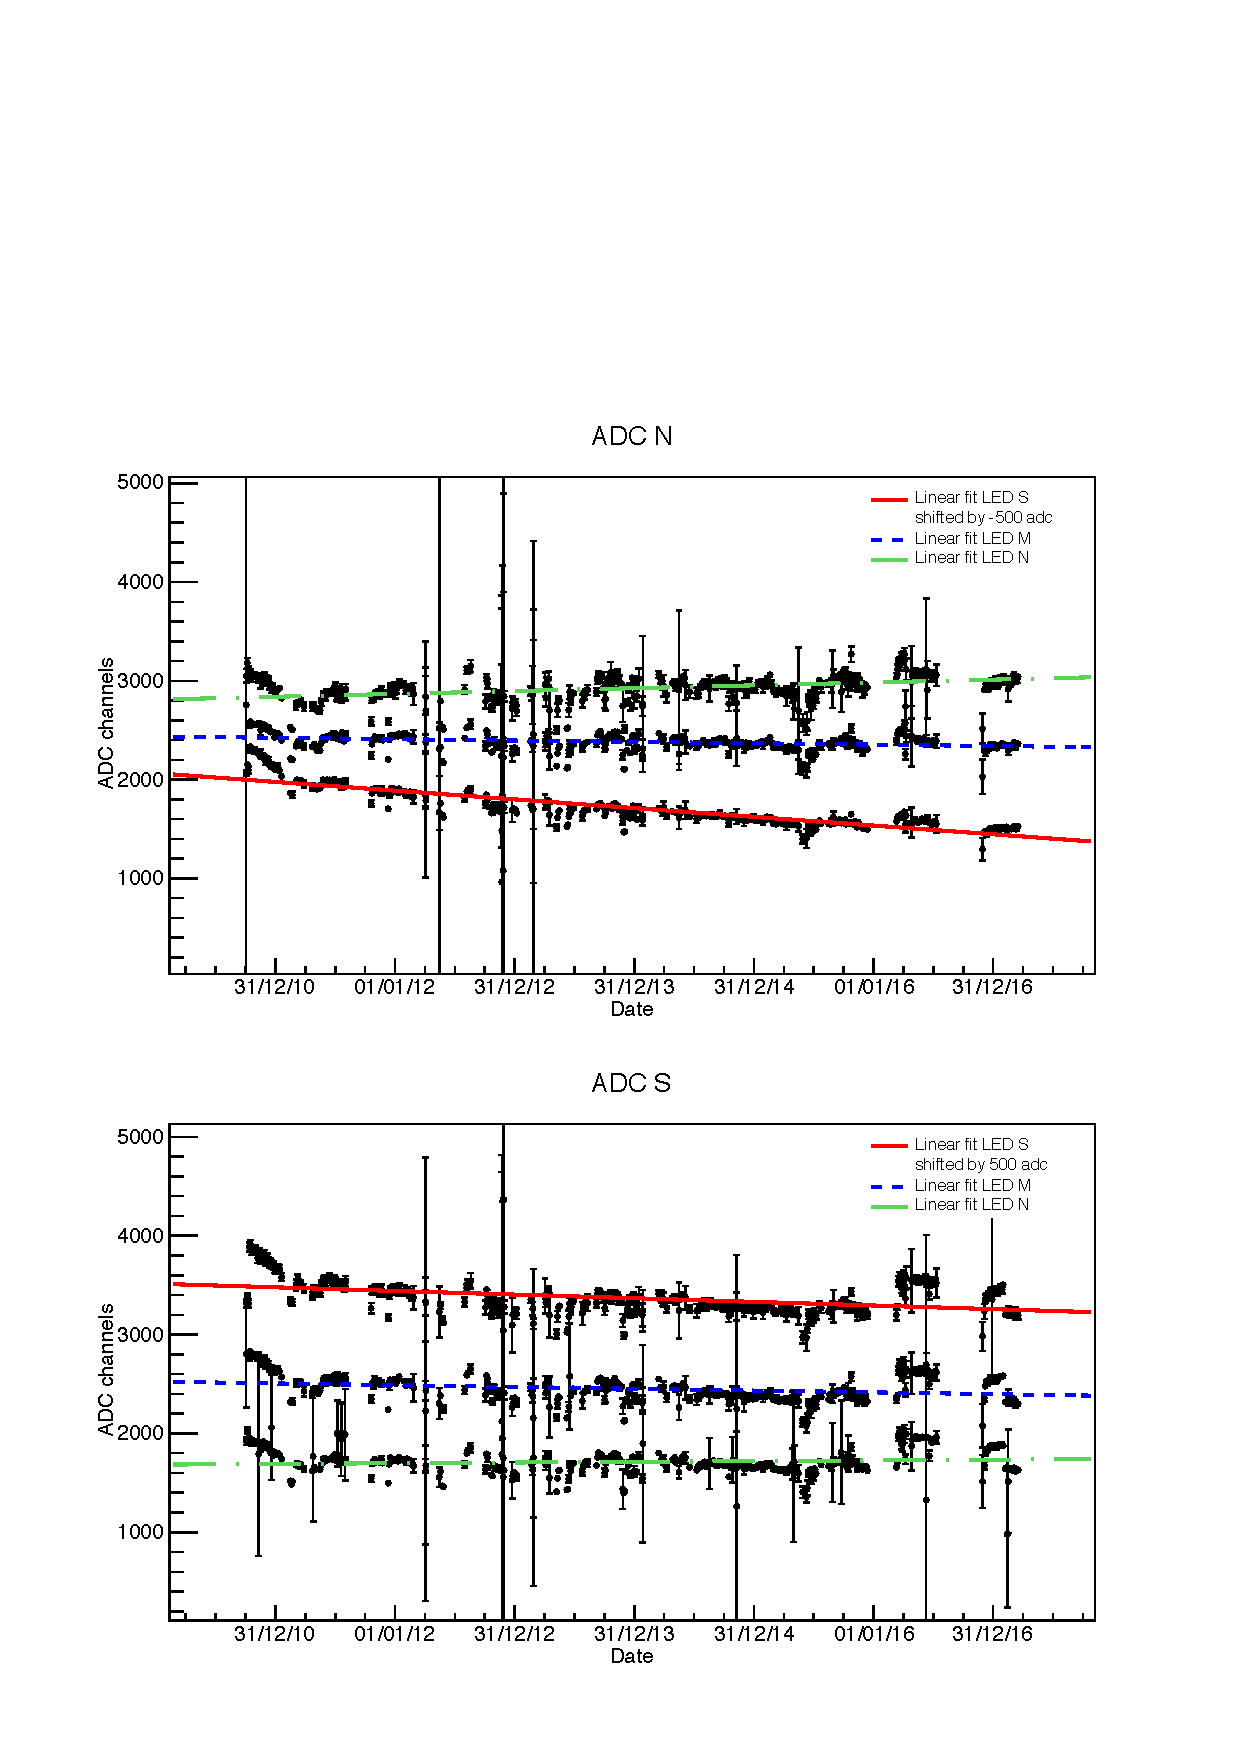
\includegraphics[width=\textwidth{}]{./fig/M8LED.pdf}
  \caption{\textbf{ADC mean values of LED signals over time in Module 8.}} The energy deposit of LED signals in ADC channels from Run70 to Run138 are plotted separately for 2 PMT groups (north in upper chart, south in lower chart). The trend of ADC values of different LEDs over time are approximated by linear fits: the green line (LED north), the blue line (LED middle), and the red line (LED south). For clarity when displaying here, the signals of the south LED are decreased by 500 channels in upper chart and increased by 500 in lower chart.
  \label{fig:M8LED}
\end{figure}

As can be seen in the figure, the mean ADC values of the two off-center LEDs differ about 500 to 1000 channels from the far end to the near end. Since M7 and M8 are only half the length of other top modules, such position dependent effects are expected to be even more remarkable in other modules.

\begin{table}[hb]
  \centering
  \caption{Slopes of the linear regressions of 3 LEDs in M8. The first uncertainty is the statistical uncertainty from the linear fit, the second is the estimated systematic uncertainty. }
  \label{tab:led}
  \begin{tabular}{c c c c}
  \toprule
        & \multicolumn{3}{c}{slope in channels/month} \\
        & LED S   & LED M  & LED N \\
  \midrule
  ADC N & $-7.26\pm0.05\pm4.32$ & $-1.13\pm0.05\pm1.06$ & $+2.37\pm0.07\pm3.12$  \\
  ADC S & $-3.02\pm0.07\pm5.50$ & $-1.49\pm0.06\pm2.92$ & $+0.59\pm0.05\pm2.74$  \\
  \bottomrule
  \end{tabular}

\end{table}

In fig.\ref{fig:M8LED}, the error bar of a single data point is the statistical uncertainty given by the gaussian fit. Since most LED events in one fire series have good gaussian form, the statistical uncertainty is mostly much smaller than the total uncertainty. Several other effects lead to the fluctuation of the ADC value, for example, the switch-on effect of electronics after a long pause. Consequently, the systematic uncertainty can only be approximated. The result of the linear fits are listed in Tab.\ref{tab:led} with uncertainty. The systematic uncertainty of the slope is estimated by fitting the first half, the middle half, and the last half of the total time period and taking the difference of the maximum and minimum slopes. \\
For example, the slope of LED S measured in the northern PMT group of M8 is estimated to be $k_{1}=-12.39\pm0.15$ channels/month for the first half (2010-2013), $k_{2}=-5.38\pm0.12$ channels/month for the middle half (2010-2013) and (2012-2015) and $k_{3}=-3.75\pm0.32$ channels/month for the last half (2014-2017). The systematic uncertainty is thus given by the half the difference between $k_{1}$ and $k_{3}$: $\Delta k_{\mathrm{sys}}=\SI{4.32}{channels/month}$.

\subsection{Discussion of the results}

Various effects could lead to the decrease or even increase of the mean ADC value of LED events. First, the transparency of plastic scintillator decreases over time. Assuming that such ageing effect is homogeneous in one module, the loss of light output depends on the distance from the event position to the PMT group. This leads to roughly the same decrease for events that have same track length to the PMT group, e.g. LED N to ADC S and LED S to ADC N. Second, the PMTs as well as the junction of scintillator module and PMT group have aged individually, which leads to different variation of ADC values at two ends of a module. Last, the light output of an LED may vary over time and thus leads to the simultaneous change of measured values in two PMT groups.

The slopes of middle LED in two ends of M8 are about the same, implying that the two PMT groups of M8 have aged similarly. Therefore the ageing effect of the plastic scintillator can be estimated by subtracting the slope of the same LED at the near end from the one at the far end. \\
For LED S, this value is $\Delta{}_{\mathrm{LED\,S}}=\SI{-4.2}{channels\per month}$ and for LED N $\Delta{}_{\mathrm{LED \,N}}=\SI{-1.8}{channels\per month}$. The values vary much from each other but still lie in the region of estimated uncertainty. This implies that the systematic uncertainty is indeed large, as these two values are expected to be the same for a homogeneous ageing of the scintillator.

Furthermore the decrease is noticeably more rapid at earlier stage (about 2010-2011) and becomes flat later. The reason can be that the transparency loss of scintillator is not linear over time. The assumption of a linear trend is thus only an approximation.
Averaging over time, the decrease due to ageing of plastic scintillator is estimated to correspond to  $\approx \SI{3}{channels\per month}$. During the total period of experiment (about $\SI{90}{months}$), the change of ADC values caused by scintillator ageing is about $\SI{250}{channels}$ for M8. Given the start values of $\approx$2500\,ch for LED pulses, this corresponds to roughly 10\% loss in light output for an event at a distance about 1.65\,m from a PMT group.

The same procedure is applied on other three modules M7,M15 and M16 and shows similar results. Since other modules are longer then the four modules, the decrease of ADC values are expected to be more significant. This is in fact the case, see table \ref{tab:mpv}. Consequently, the detection efficiency of a individual module reduces, especially for events to be measured in the far PMT group, as the transportation length of light is longer.

\subsection{Conclusion}

To conclude, the analysis of LED events shows that the gain of PMT groups has decreased. Although the change is negligible for a short period, it becomes significant accumulating over the long time period of seven years.

In this chapter, LED events are used to investigate the ageing effect of the muon-veto scintillator modules. This method has the advantage that the selected events are pure LED events, unlike the selection of muon events which always contains certain backgrounds. In addition, the measured energy spectrum of LED events is gaussian distributed and the mean ADC values can be easily determined. \\
Moreover, every measured LED event can be associated to a certain LED, or correspondingly a certain position. As described above, this allows to separate the effects of different sources on the ageing of a module. For example, the difference of mean ADC values of LED N in two PMT groups gives a measure of the transparency loss of the scintillator. Though the position of muon events can also be reconstructed by the difference of two TDC values, the ageing effects of different sources cannot be reliably separated due to the low statistics and the wide energy spectrum of muon-induced events.

On the other hand, this method using LED events also has its limitations. First of all, the result obtained here only shows qualitatively that the modules have aged. It gives little information on the actual effect on the change of the muon detection efficiency, which is essential for the experiment. Also, as mentioned before, only four extra modules are equipped with LEDs. The other modules cannot be investigated using this method. To achieve that, muon induced events are analysed in the next chapter.





%discussion, pro and cons of LED vs muon events ...
%relation to muon efficiency

    \chapter{Determination of the long term stability using muon events }
    \label{chap:ana_muon}
    % chapter5.tex
% Muon events, threshold analysis
Analysis of LED events can only be applied on the four extra top modules. To determine the stability of the total \mvs, aging of all modules are investigated. In this chapter, the muon-events are selected and analysed. Additionally, the effective threshold of each module is determined using an independent method, which allows to estimate the change of the detection efficiency of the modules.

\section{Analysis of muon events}

\subsection{Selection of muon-veto data}
All the data from Run70 (Aug 2010) to Run138 (Mar 2017) are investigated in the following analysis. Since the goal of the analysis is to  several cuts must be applied on the data to ensure a stable condition of the system during the investigated time period and to decrease
First, data taken when the \mvs{} was not fully closed are cut. As described in \ref{sec:muon-setup}, two lasers measure the position of the upper part of the muon-veto every 15 minutes. Time periods when the gap size deviates more than 5 cm from the closed configuration are cut, since the \mvs{} is either fully closed or fully opened. When the system is opened, the detection efficiency of through-going muons decreases and the background rate increases largely, which will lead to a increase of low energy events and .

When the \mvs{} is closed, most muons go through at least 2 modules. Therefore a coincidence in 2 distinct modules is required for selecting muon events. An energy deposit with full information in each module is required--i.e.\ both TDCs and ADCs have non-zero values. It respectively reduces events caused by secondary particles or natural backgrounds since they mostly deposit less energy than muons. By applying this cut criterium, the event rate in one module is reduced to the order of $\SI{10}{events/day}$.

\subsection{Data analysis}
As mentioned in section \ref{sec:muon-working}, the spectrum of muon energy deposit in modules can be described by a Landau distribution. The ADC values of muon events in a time period are fitted with a Landau distribution and the obtained MPVs in different time periods are used to analyse the long term behaviour of the \mvs. The fig.\ \ref{fig:Landau_M6} shows an example of the Landau fit. Since the muon event rate is low, the obtained ADC values in a two months period are combined to perform each fit.

\begin{figure}[ht]
  \centering
  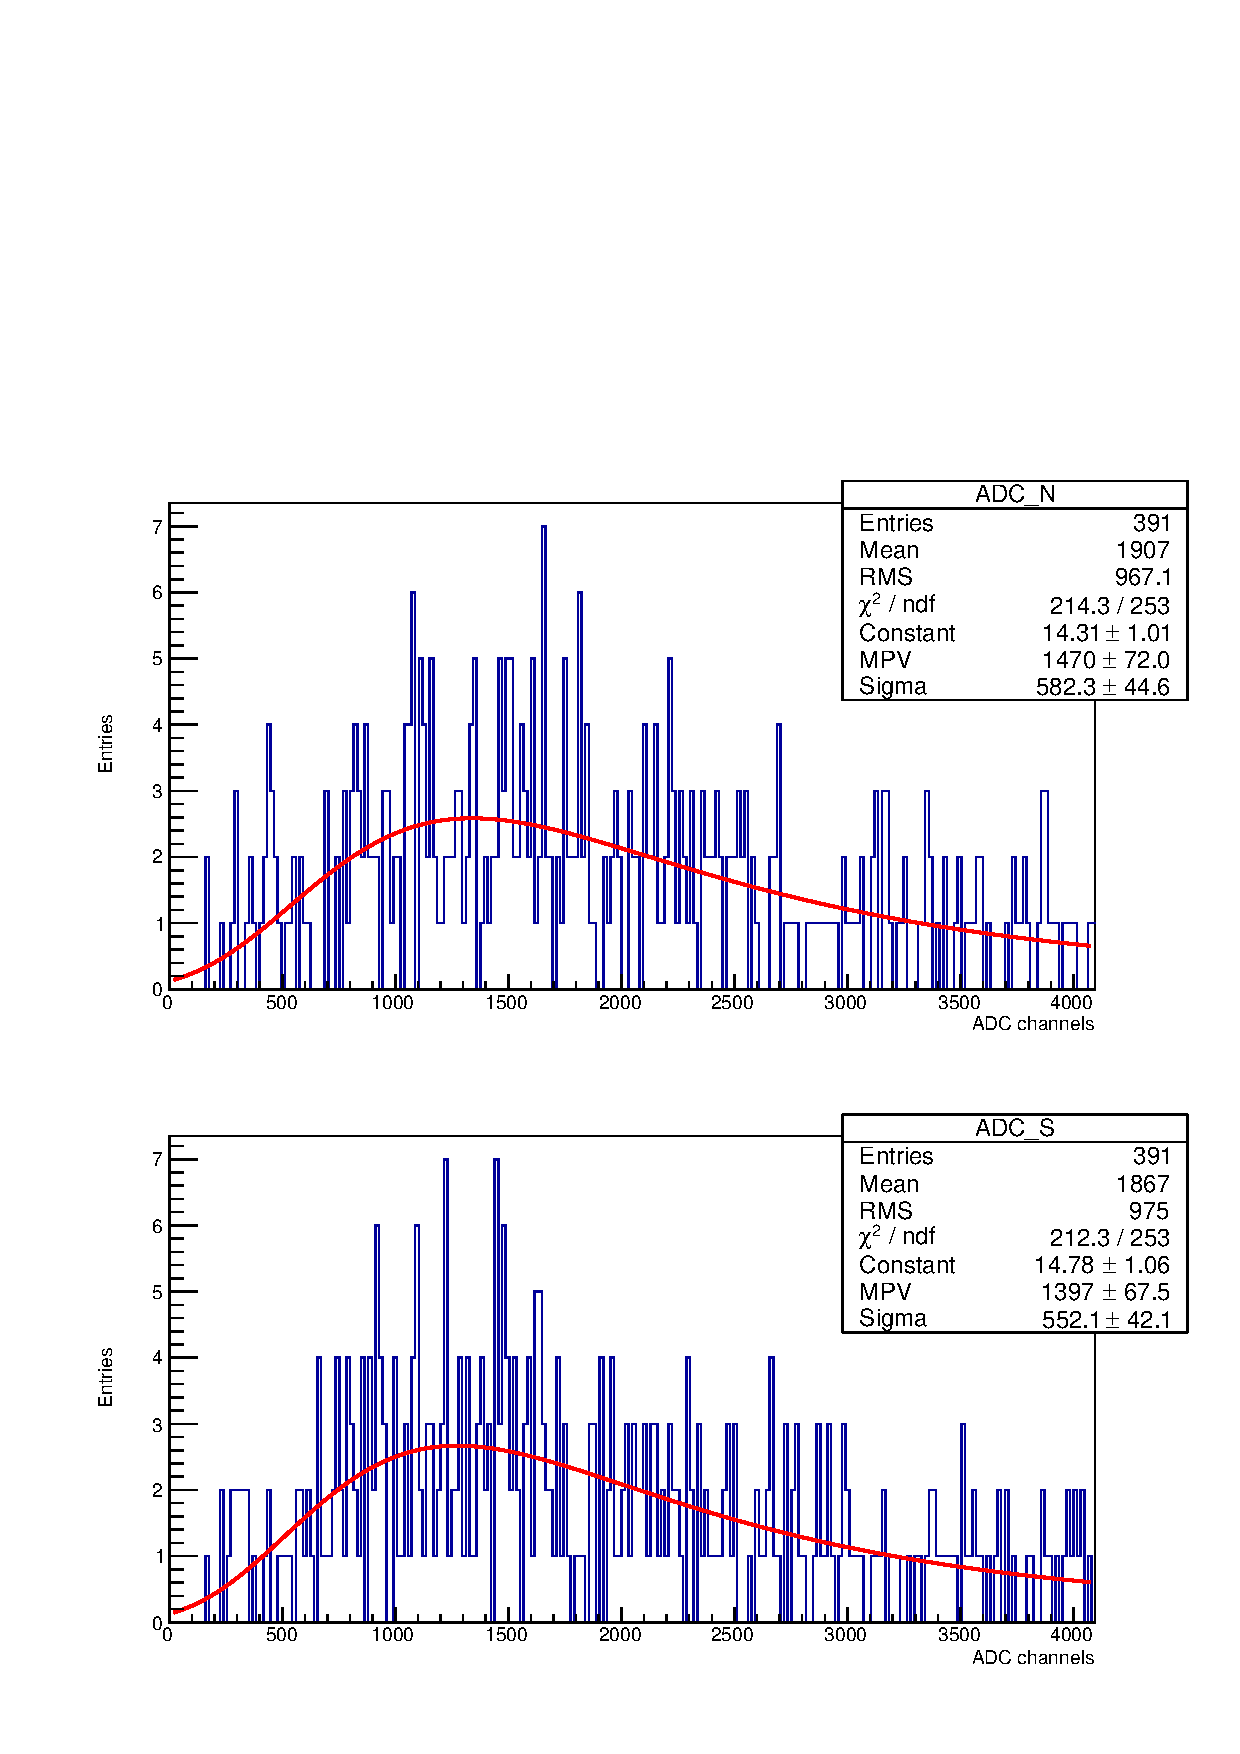
\includegraphics[width=0.6\textwidth{}]{./fig/LandauFitM6.pdf}
  \caption{Example of a Landau fit in M6. The fit uses a log likelihood method in ROOT.}
  \label{fig:Landau_M6}
\end{figure}

The MPVs obtained from the Landau fit are plotted over time (see fig.\ \ref{fig:MPV}). Some time periods with too few entries due to the system shutoff are excluded, since no reliable Landau fit can be performed. It is to be noticed that the data points have rather large uncertainty, which is partially due to the smeared spectrum. As explained before, the light output is strongly position dependent and decreases exponentially with the path length from the interaction point to the PMT group. Furthermore, there are some sudden changes of the MPVs. The reason could be the restart of the \mvs{} after operations.

\begin{figure}[hp!]
  \centering
  \begin{subfigure}{0.6\linewidth}
    \centering
    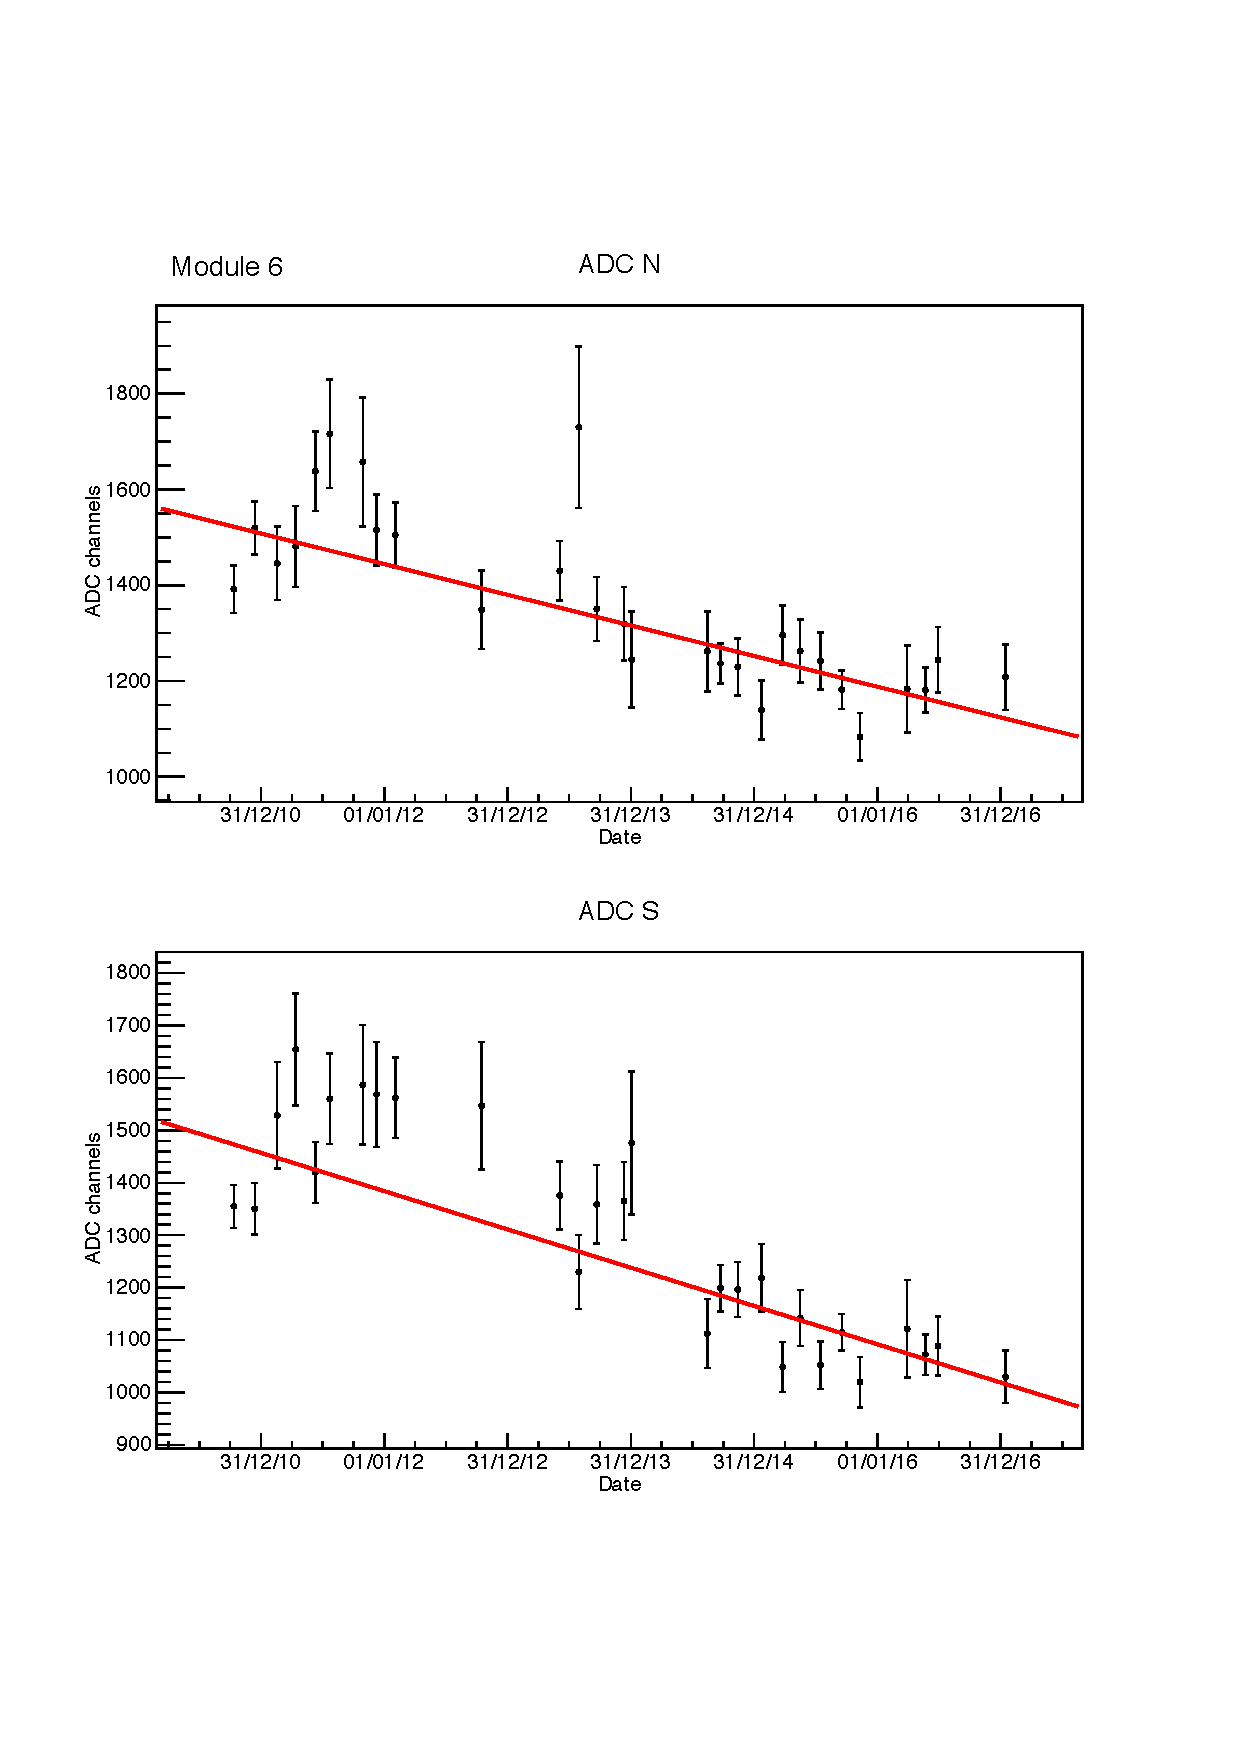
\includegraphics[width=\linewidth{}]{./fig/M6mpv.pdf}
    \caption{}
    \label{fig:MPV_M6}
  \end{subfigure}
  \begin{subfigure}{0.6\linewidth}
    \centering
    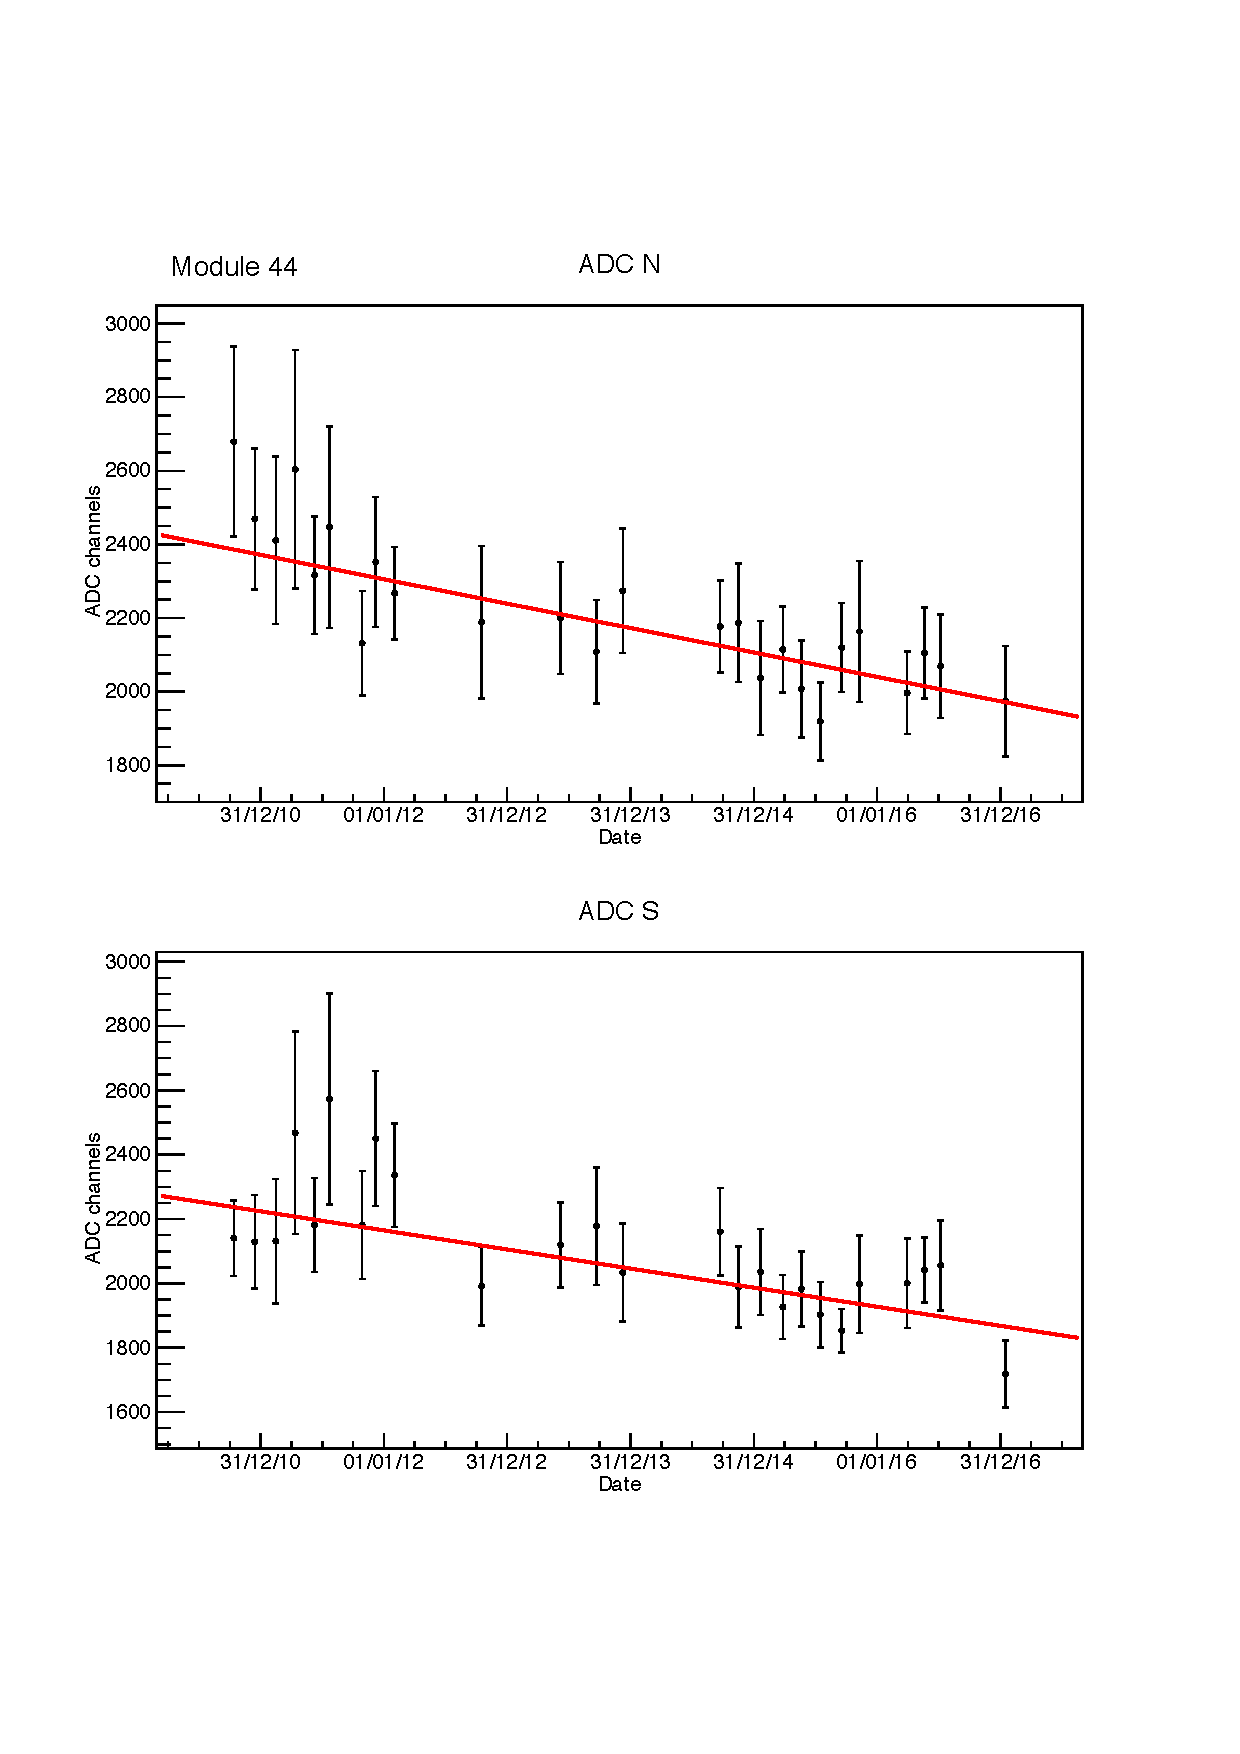
\includegraphics[width=\linewidth{}]{./fig/M44mpv.pdf}
    \caption{}
    \label{fig:MPV_M44}
  \end{subfigure}
  \caption{MPVs over time with linear fits in two example modules. The two upper figures show the MPVs in M6 (top module) and the two lower figures show the MPVs in M44 (bottom module).}
  \label{fig:MPV}
\end{figure}

%
%\begin{figure}[htb]
%  \centering
%  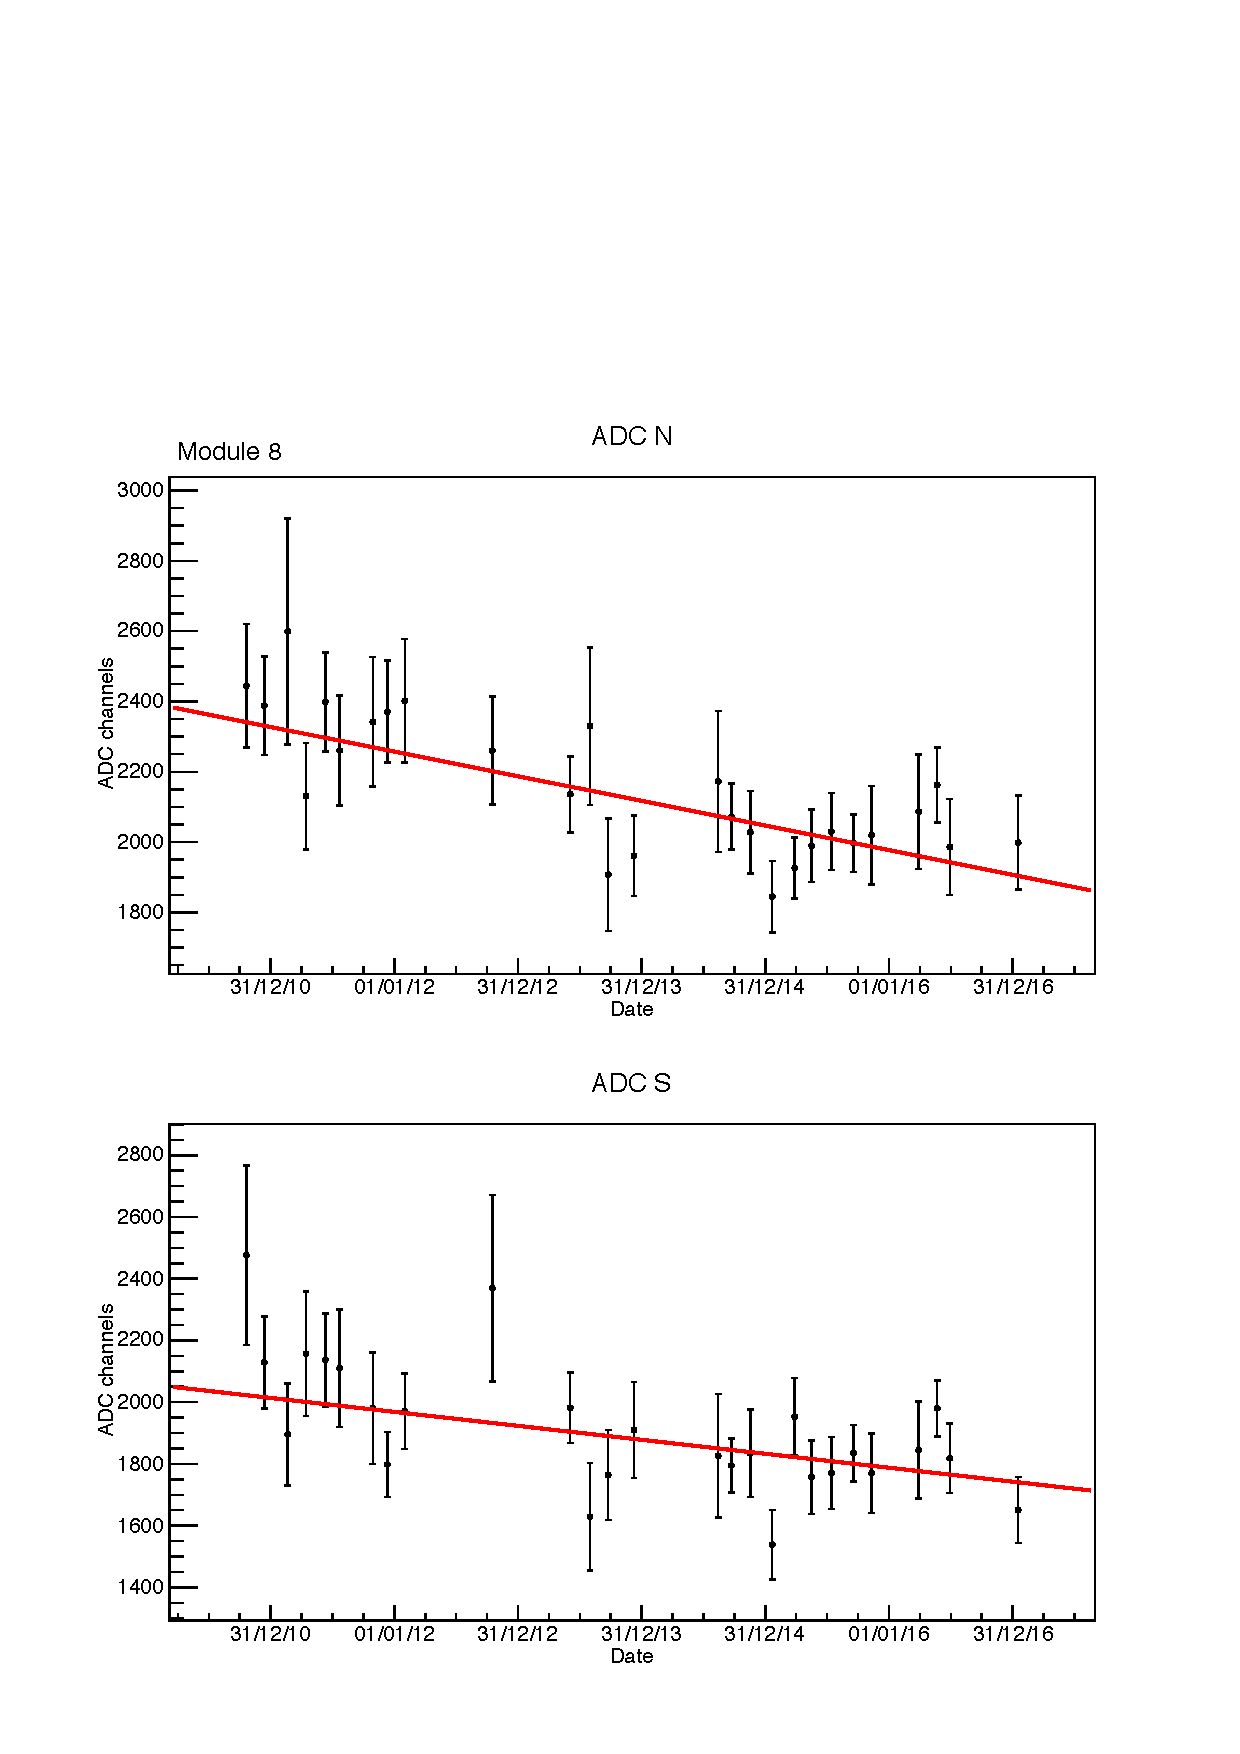
\includegraphics[width=0.6\textwidth{}]{./fig/M8mpv.pdf}
%  \caption{MPVs over time with linear fit in M8.}
%  \label{fig:Landau_M8}
%\end{figure}

\begin{table}[hb!]
  \centering
  \caption{Slopes of the linear regressions of MPVs in example modules M6, M8 and M44. The statistical uncertainty is obtained from the fit program in ROOT. }
  \label{tab:mpv}
  \begin{tabular}{c c c c}
  \toprule
  Module & \multicolumn{2}{c}{slope in channels/month} \\
         & ADC N & ADC S \\
  \midrule
  M6  & $-5.44\pm1.34$ & $-4.87\pm1.12$ \\
  M8  & $-5.26\pm0.52$ & $-6.00\pm0.46$ \\
  M44 & $-5.76\pm3.71$ & $-3.71\pm1.12$ \\
  \bottomrule
  \end{tabular}
\end{table}

The change of the MPVs are again approximated by a linear regression and the obtained slopes are listed in tab.\ \ref{tab:mpv}. It can be seen that the slopes for two ends in a single module don't vary much from each other, which means that the aging of plastic scintillator is as expected almost symmetric and the electronics of two PMT groups have also aged similarly.

The value obtained in M8 is also listed for comparison with the result from LED data. The decrease of the MPVs is larger than the one of ADC mean values of middle and northern LED events and lies in the uncertainty regions of southern LED events. The abnormal increase of ADC mean values of LED S in M8 (see tab.\ref{tab:led}) is not to be found in the data obtained from muon events. Thus it can be concluded that the problem is merely due to the behaviour of the LED but not the scintillator module.
Despite the various effects that may lead to a sudden change of the ADC value, the MPVs of the Landau spectrum in all 46 modules show a general decrease of several hundred ADC channels since 2010.



\section{Determination of the detection efficiency}
The analysis above shows that the gain of the PMT groups have decreased remarkably since the start of the experiment. However, it doesn't provides a direct measure of the change of the muon detection efficiency. To estimate the detection efficiency, the knowledge of the trigger threshold of each module is needed. Before the experiment, the scintillator modules have been calibrated using cosmic muons \cite{Hab04}. Due to the aging effects of the modules, the trigger threshold must be determined again. As the muon flux in the underground laboratory is reduced significantly, the cosmic muons cannot be used for calibration anymore. In this section, an alternative approach to determine the trigger threshold is described. The detection efficiencies in different time periods are derived using the obtained threshold values.

\subsection{Effective trigger threshold}
As discussed in section \ref{sec:muon-working}, there are two thresholds in the measurement of \mvs. One is a digital conversion threshold, which is typically set to 120\,ADC channels. The influence of digital threshold on the muon detection efficiency can be neglected, because the MPVs are typically above 1000\,ADC channels and the Landau distribution falls quickly towards the low energy region.

The trigger threshold, on the other hand, is relevant for the following analysis. It is a hardware threshold which is set to 150\,mV. Only the pulse with an amplitude above this value triggers the data acquisition. Although the hardware threshold is set to same voltage in each module, the value in ADC channels depends on the gain of the individual PMT groups. Thus the value of trigger threshold is different in each module. Additionally, it depends on the shape of measured pulse, since the ADC value is the integral of a signal. For example, a flat pulse has a larger energy deposit than a steep pulse with same amplitude. The pulse shape also depends on the light propagation and is thus position dependent. Therefore, the effective trigger threshold is expected to be a curve instead of a step function.

The efficiency of a module is a function of energy, which is low for low energy deposit and is expected to be 100\% in high energy region. It is similar to the behaviour of an error function:
\begin{equation}
  \mathrm{erf}(x)=\frac{2}{\sqrt{\pi}} \int_{0}^{x} \! e^{-t^{2}}\, \mathrm{d}t
\end{equation}
It describes the convolution of a Heaviside function $\Theta(x)$ with a Gaussian distribution. By shifting and rescaling, the error function is able to imitate the behaviour of the actual detection efficiency curve at the threshold. It is characterised by two parameters, the effective threshold $E_{\mathrm{thr}}$ and the standard deviation $\sigma$. The effective trigger threshold is defined as the ADC value where detection efficiency is 50\% and the $\sigma$ describes the smearing effect of the spectrum.

\subsubsection*{Method of effective trigger threshold determination}

When a module is triggered, all the non-zero signals in the \mvs{} are stored. It is therefore possible to analyse the the events for a certain module I even if they don't trigger the module I. For the analysis of one PMT group X in module I, the ADC values of all the events that have triggered another module J are stored in histogram H1. In contrast to the condition of muon selection, which requires both non-zero TDC values, the trigger condition of a PMT group X used in the following analysis requires only that the TDC on the same side has a non-zero value. Requiring both TDC channels will introduce a dependency on the PMT group on the other side, while the trigger threshold is determined separately for two ends of a module. The events with one TDC trigger are stored in histogram H2. The efficiency of one PMT group is determined by the division of H2 and H1.

\begin{figure}[ht]
  \centering
  \begin{subfigure}{0.7\linewidth}
    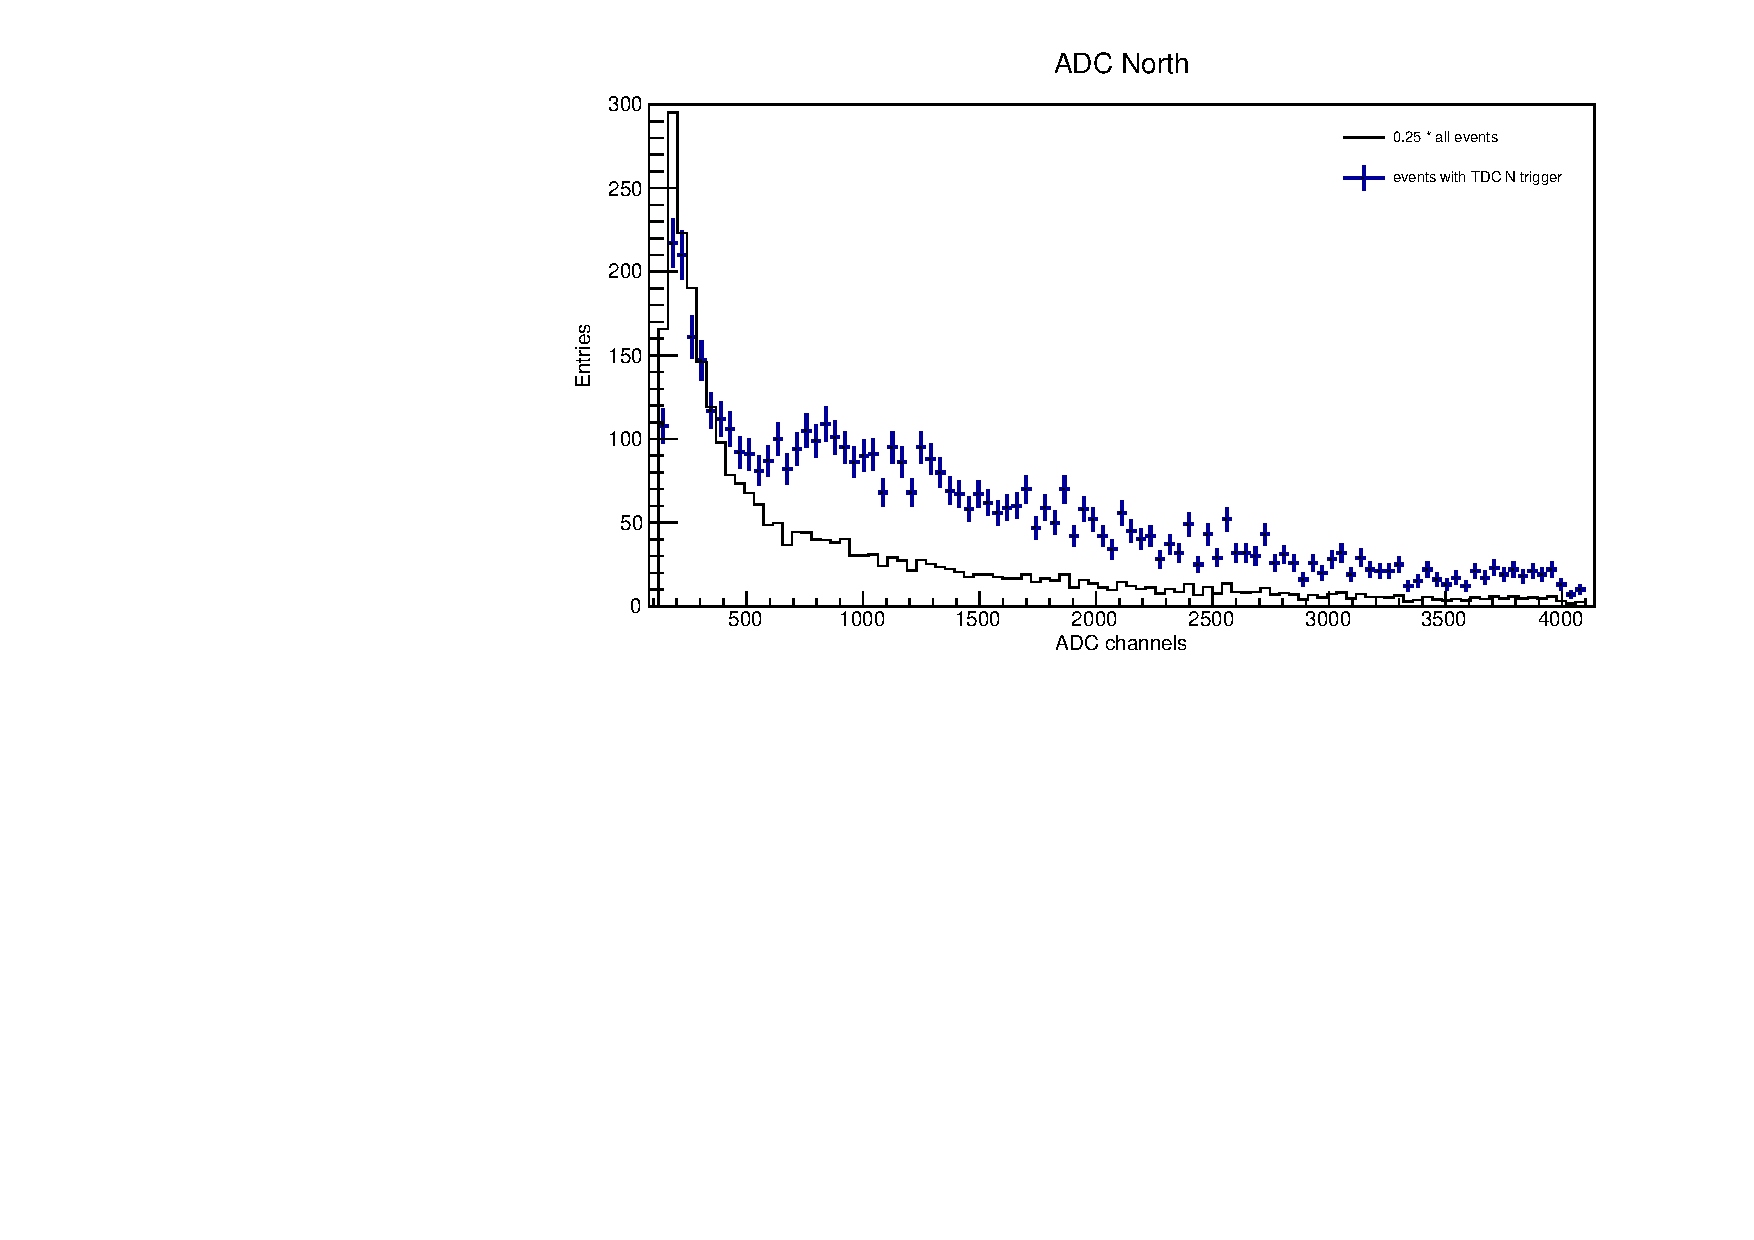
\includegraphics[width=\linewidth{}]{./fig/M6AdcNorth2Histo.pdf}
    \caption{Example of the spectrum with and without trigger condition of ADC N in M6. The data points (blue) are events which satisfy the trigger condition in the same end (Northern PMT group). The spectrum of all events (black) are scaled by a factor of 4.}
    \label{fig:2HistoM6}
  \end{subfigure}
  \begin{subfigure}{0.7\linewidth}
    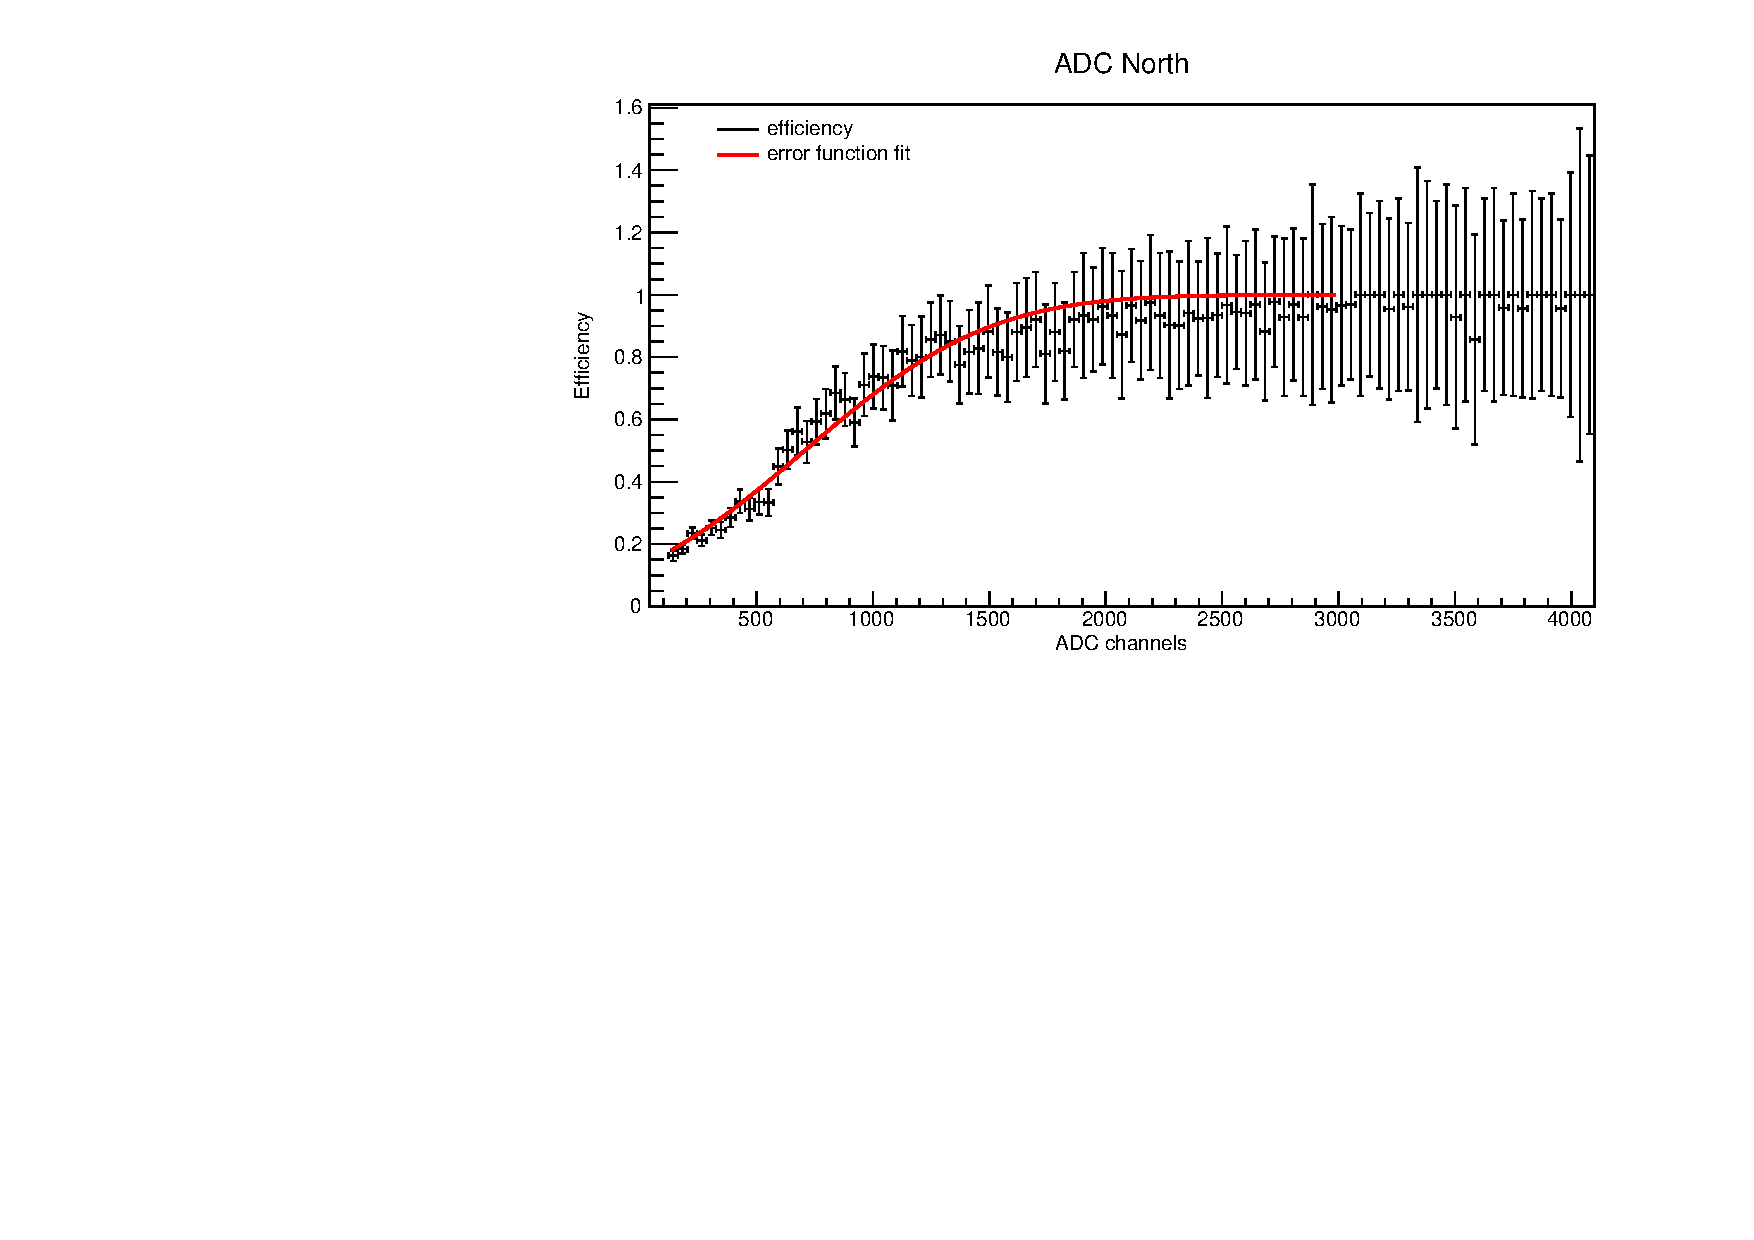
\includegraphics[width=\linewidth{}]{./fig/M6AdcNortheff_late.pdf}
    \caption{Histogram of events triggering the PMT group on the same side divided by all events with error bars (black) and the error function fit (red).}
    \label{fig:eff_lateM6}
  \end{subfigure}
  \caption{Example of the method to determine the effective trigger threshold of a PMT group.}
  \label{fig:threshold_example}
\end{figure}

Fig.\,\ref{fig:threshold_example} shows an example of this method. The events that triggered one PMT group are plotted with all events. As expected, the detection efficiency increases with ADC values and goes toward 100\%. As can be seen in the figure, the increase is slightly asymmetric: it is more rapid at first and is then flatter. The estimation with an error function is therefore conservative for low energy events and optimistic for high energy events.

The effective trigger threshold in ADC units are calculated for each PMT group in different time periods. To increase statistics, several runs are combined to perform the error function fit. Run 70-79 (year 2010) are investigated for the early time period and Run 124-138 (year 2015-2017) for the late time period. The results are listed in tab. \ref{tab:efficiency_short} in the following section.


\subsection{Detection efficiency of a module}
In addition to the above criteria, events with a coincidence in adjacent modules are excluded. These events have a higher probability to be induced by secondary particles or grazing muons. They mostly have low energy deposits, where the efficiency is also low due to the trigger threshold, and can lead to a decrease of total detection efficiency.

\begin{figure}[h!]
  \begin{subfigure}{0.5\linewidth}
    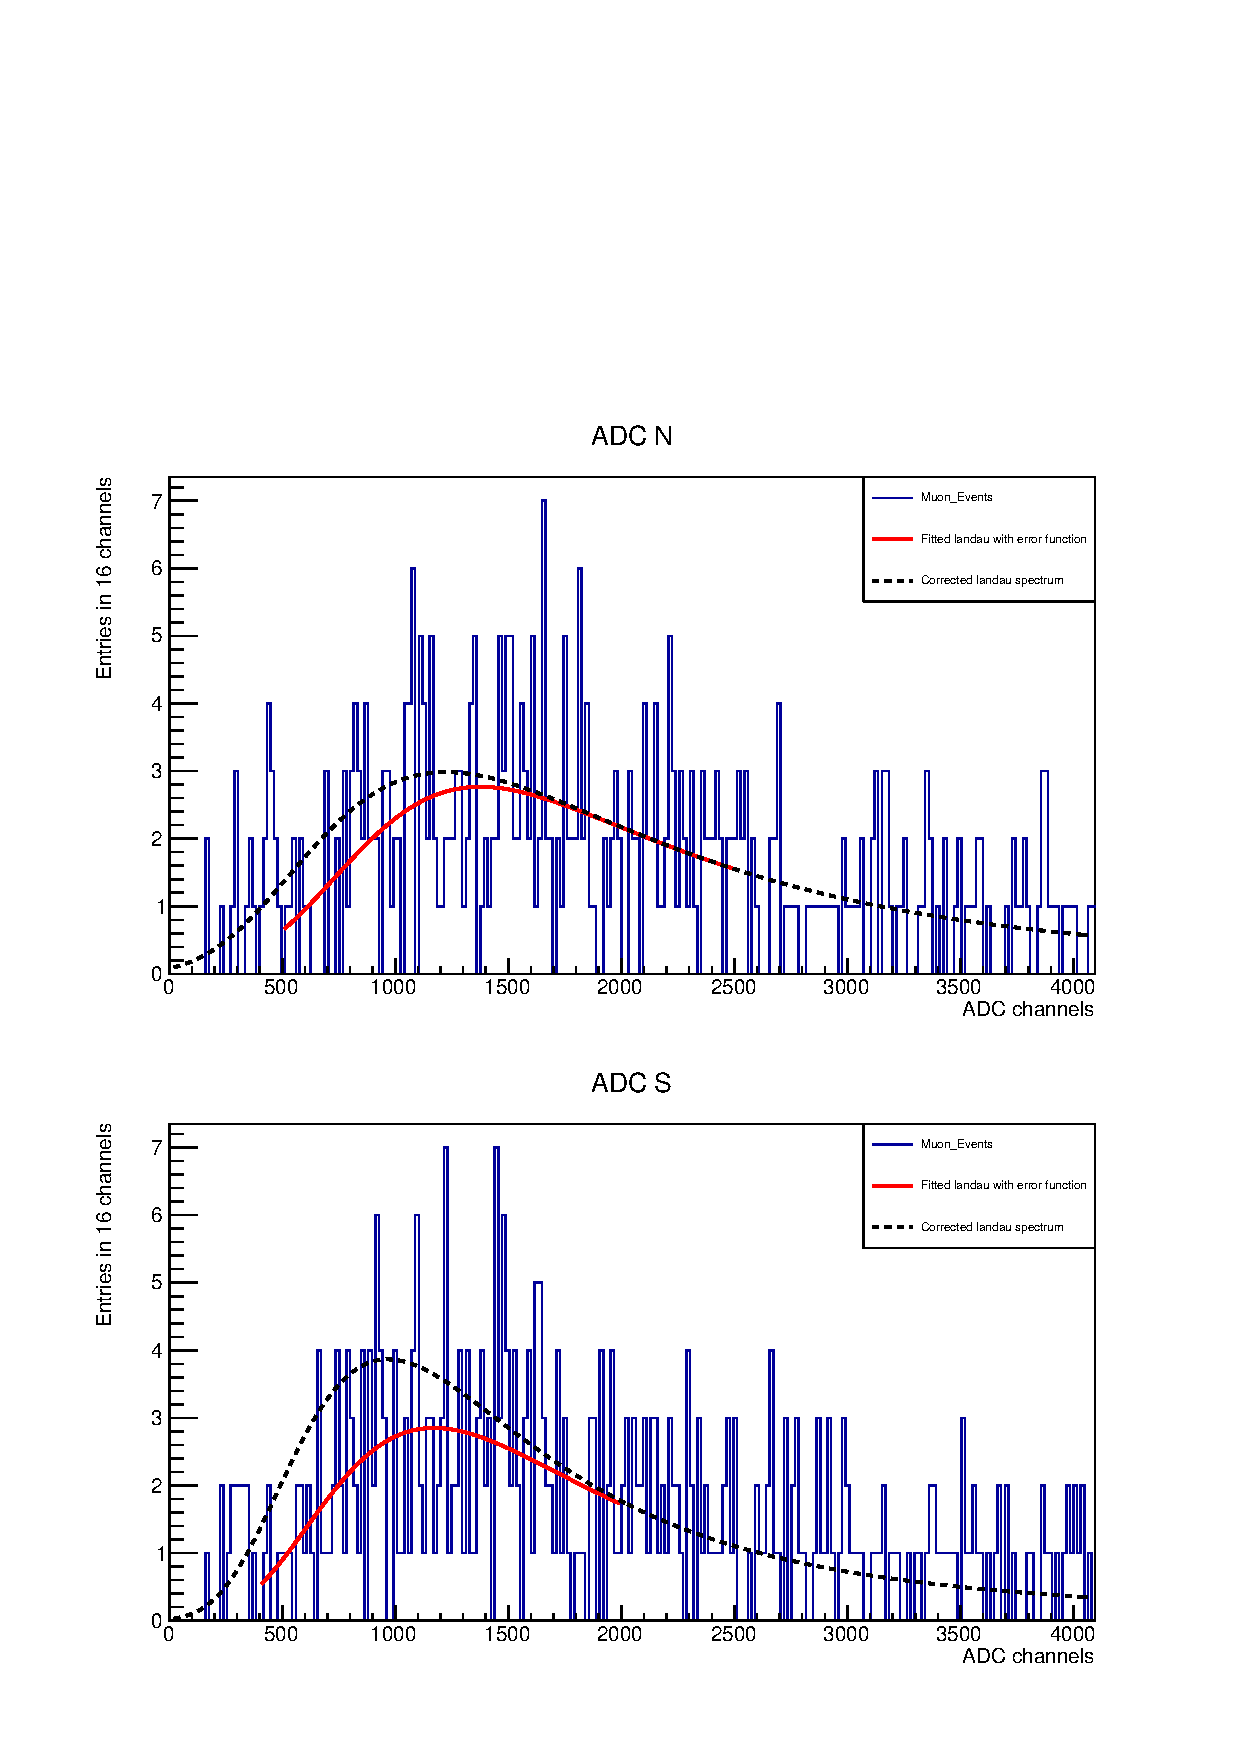
\includegraphics[width=\linewidth{}]{./fig/70M6CorrectedLandau.pdf}
    \caption{}
    \label{fig:landau_earlyM6}
  \end{subfigure}
  \begin{subfigure}{0.5\linewidth}
    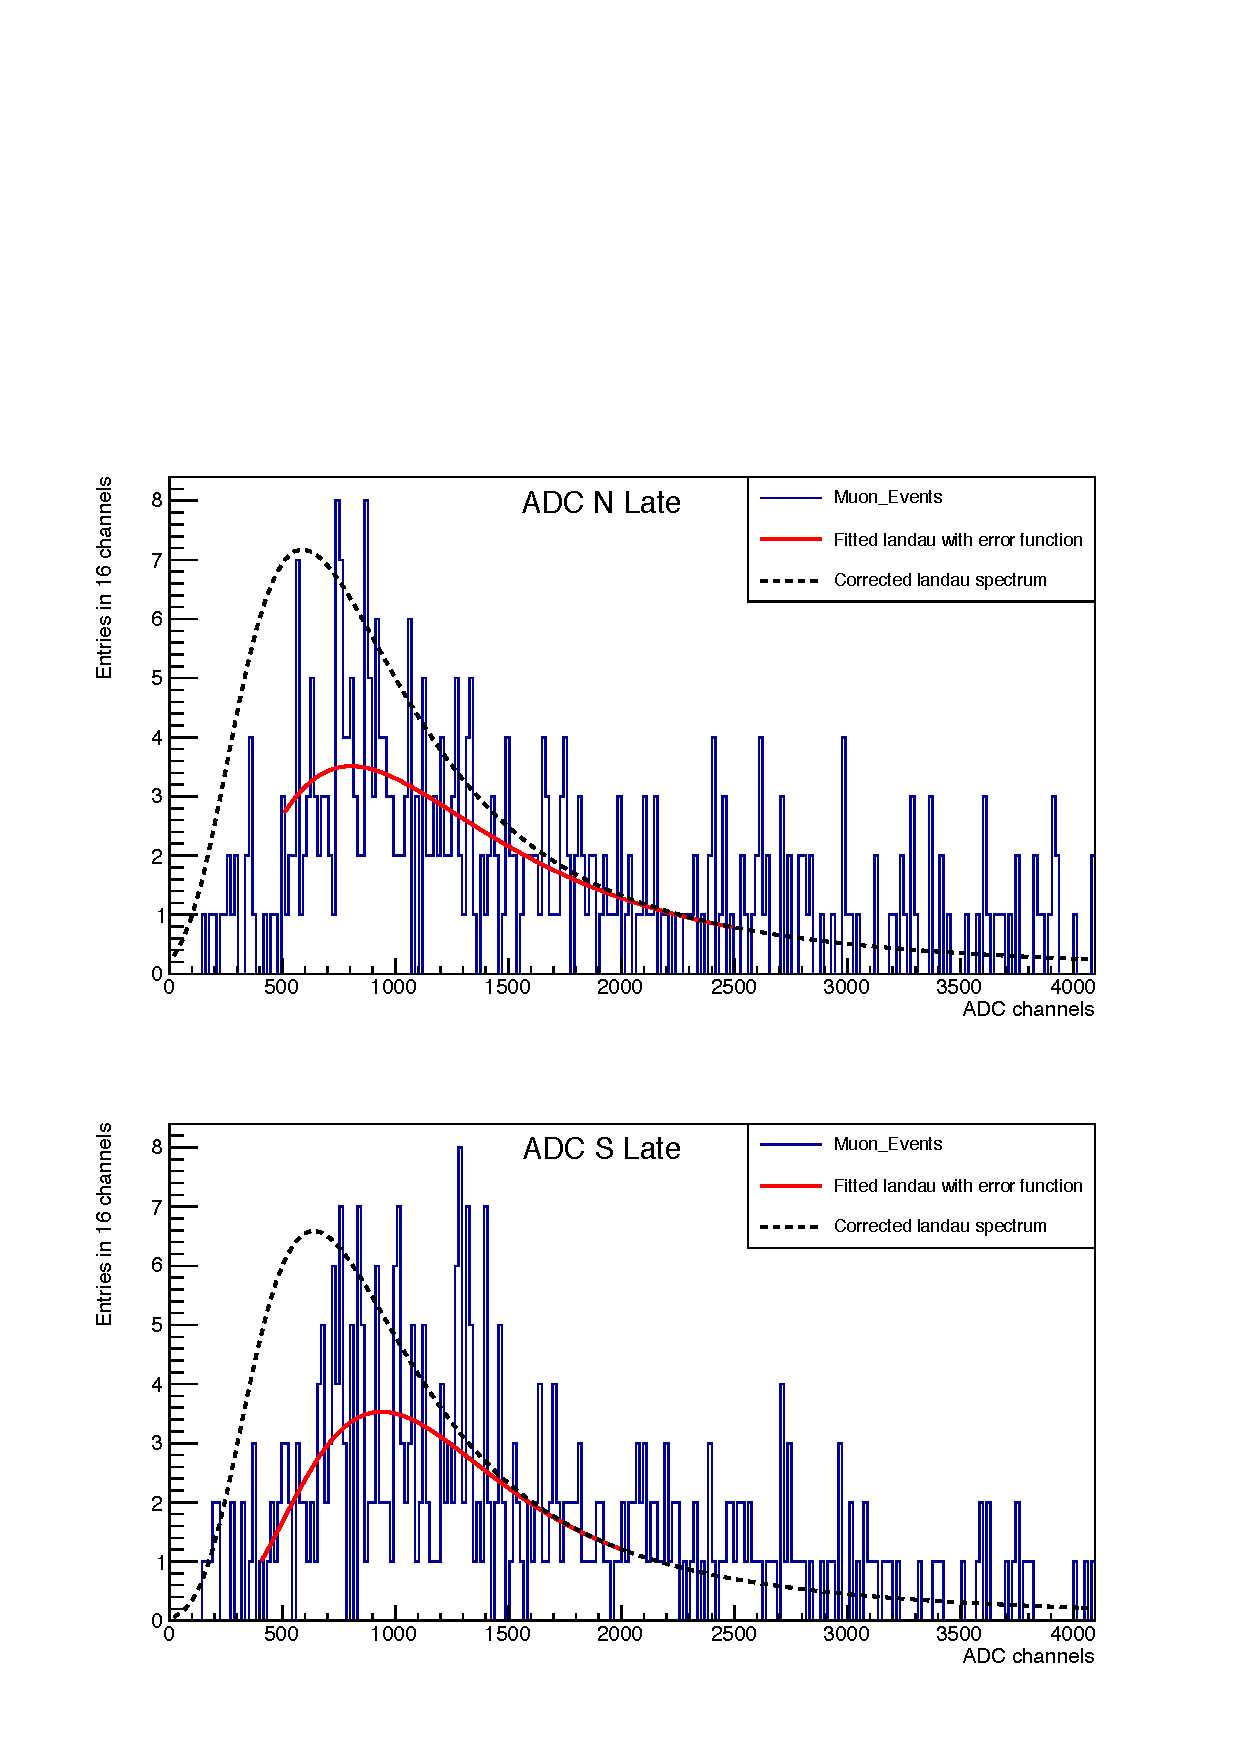
\includegraphics[width=\linewidth{}]{./fig/124M6CorrectedLandau.pdf}
    \caption{}
    \label{fig:landau_lateM6}
  \end{subfigure}
  \caption{Spectrum of muon-induced events in M6 in earlier runs (left) and latest runs (right). The spectra are fitted with a Landau distribution with an error function (red). The corrected spectrum (black, dotted) is determined by dividing the error function.}
  \label{fig:detection_M6}
\end{figure}

The muon energy deposit can be described with a Landau distribution, whereas the measured energy deposit is dependent on the response of the individual modules. Therefore, the ADC spectrum is expected to be a Landau multiplied by an error function. The selected data are fitted with this function and the corrected spectrum is given by a Landau distribution with the obtained parameters (see fig. \ref{fig:detection_M6}). The efficiency can be determined by the integral of the spectrum with and without the error function. The results are listed in tab \ref{tab:efficiency_short}.


\begin{table}[htb!]
  \caption{The trigger threshold and detection efficiency of PMT groups in selected modules (for the full table see \ref{sec:appendix}). The MPV in this table denotes the most probable value of the Landau distribution with error function. The total efficiency is estimated by the product of the efficiency value $\epsilon_{50\%\mathrm{MPV}}$ of each PMT group, which is determined by the integration from half of the MPV energy. }
  \label{tab:efficiency_short}
  \begin{tabular}{c c c c c c c c c}
    \toprule
    Module & End & MPV & Threshold & $\sigma{}_{\mathrm{erf}}$ & $\epsilon_{20\%}$ & $\epsilon_{50\%\mathrm{MPV}}$ & $\epsilon_{\mathrm{MPV}}$ & $\epsilon_{\mathrm{tot}, 50\%\mathrm{MPV}}$ \\
           &     & \multicolumn{3}{|c|}{in ADC channels} &   \\
    \midrule
    M6     & N & 1401 & 532 & 737 & 0.86 & 0.90 & 0.97 & \multirow{2}{*}{0.77}\\
    early  & S & 1256 & 615 & 712 & 0.83 & 0.86 & 0.95 &\\
    M6     & N & 872 & 707 & 627 & 0.67 & 0.71 & 0.85 & \multirow{2}{*}{0.53}\\
    late   & S & 975 & 746 & 416 & 0.60 & 0.75 & 0.94\\
    \midrule

    \bottomrule
  \end{tabular}
\end{table}



For some of the PMT groups, the spectrum cannot be fitted properly (for example fig.\). The efficiency is estimated by the other PMT group in the same module. If the fit method cannot be applied for both PMT groups, the total detection efficiency is given by the mean values of other modules on the same side.


\begin{figure}[ht]
  \centering
  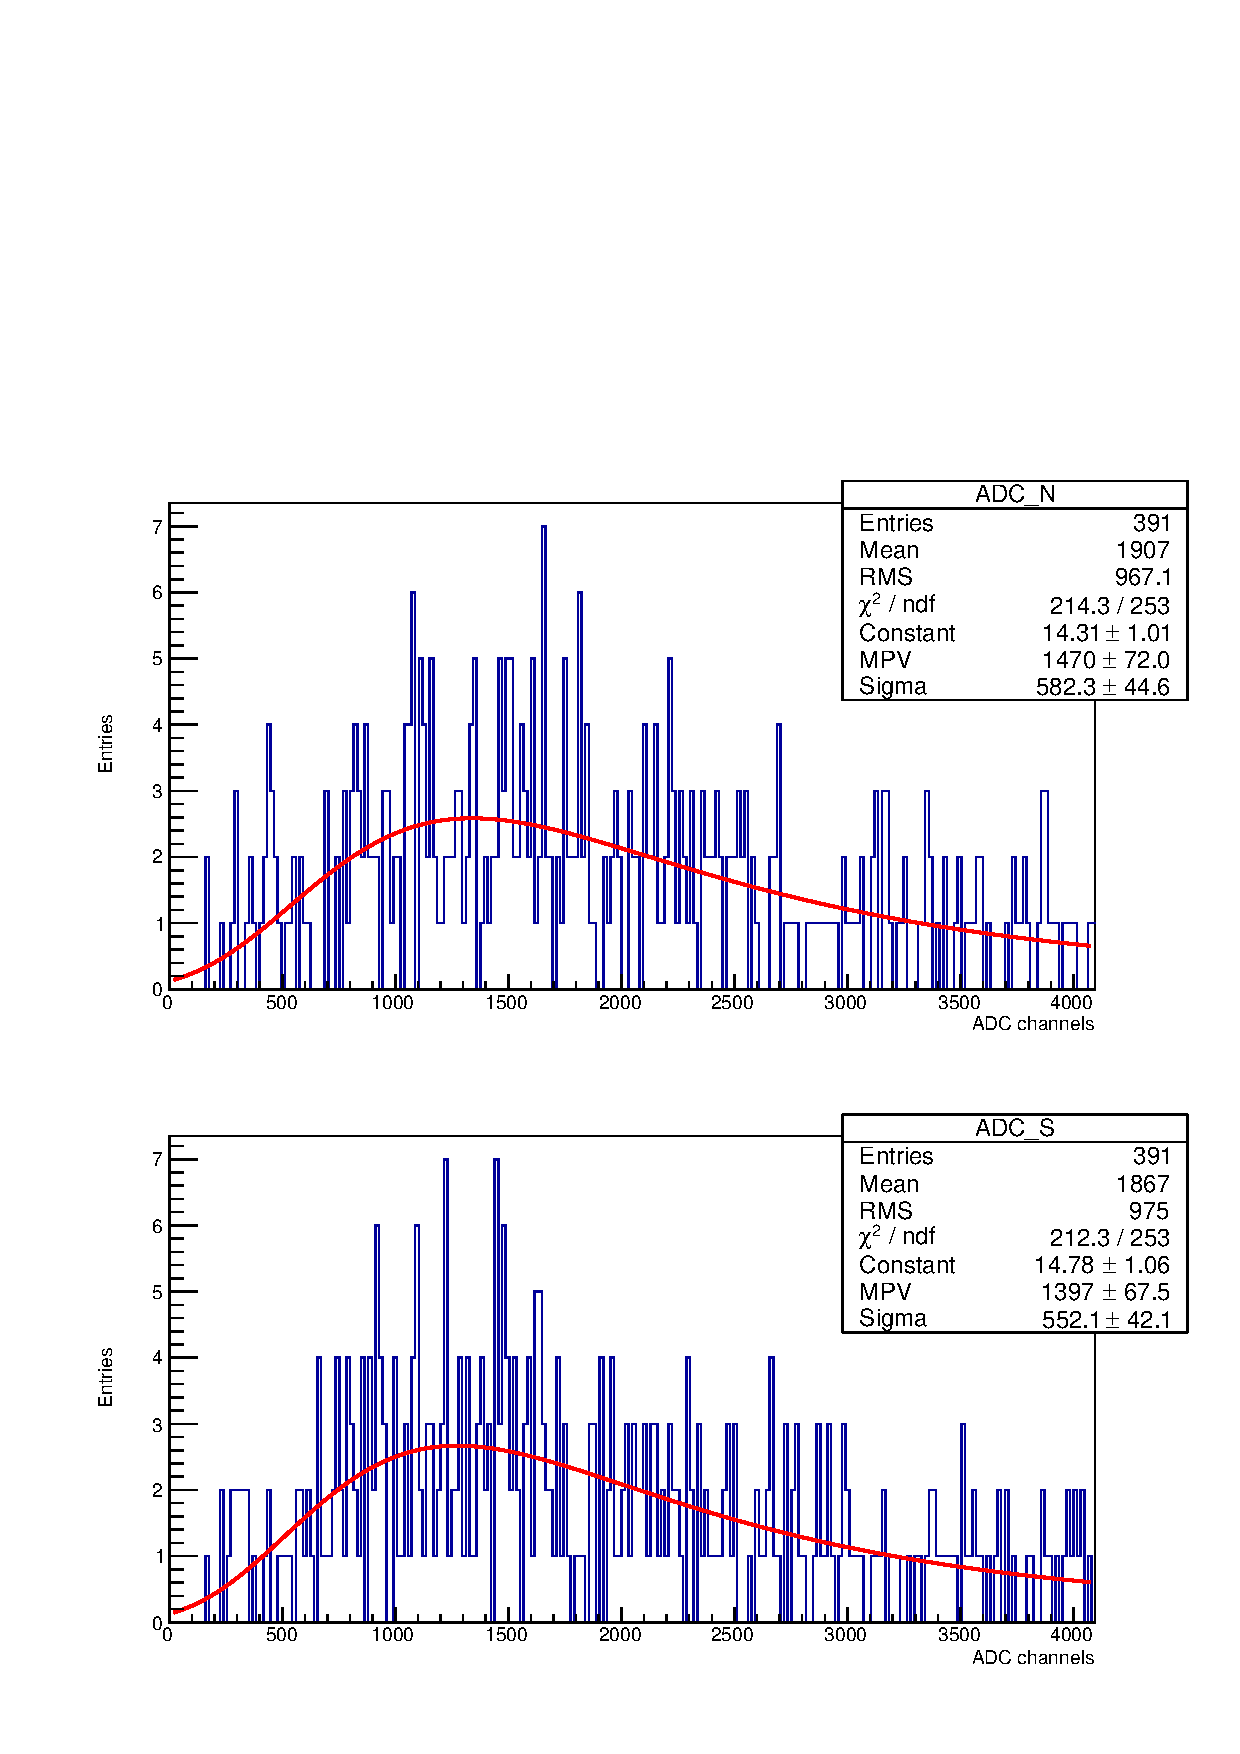
\includegraphics[width=0.6\textwidth{}]{./fig/LandauFitM6.pdf}
  \caption{Example of a failed fit in M15 in Run124-138. The efficiency is estimated by the mean value of other modules on the same side.}
  \label{fig:Landau_M6}
\end{figure}








%blahblah

    \chapter{Conclusions}
    \label{conclusion}



    %\emptychapter[3]{ROOT Routines}     % usage: \emptychapter[page displayed
                                        %        in toc]{name of the chapter}



    % appendix for more or less interesting calculations
    \Appendix
    \chapter*{\appendixname} \addcontentsline{toc}{chapter}{\appendixname}
    % to make the appendix appear in ToC without number. \appendixname =
    % Appendix or Anhang (depending on chosen language)
    \section{Detection Efficiency}
\label{sec:appendix}
some text!
%tables of efficiency
\small
\begin{longtable}{c c c c c c c c c}
  \caption{The determined trigger threshold and detection efficiency of each module in Run70-79 (2010). For some PMT groups, the spectrum cannot be fitted properly and no efficiency value can be derived. The detection efficiency is estimated by the other PMT group in the same module, or the mean value of the modules on the same side if both spectra of PMT groups cannot be fitted. } \\
  \label{tab:mpv-full}\\
  \toprule
  Module & End & MPV & Threshold & $\sigma{}_{\mathrm{erf}}$ & $\epsilon_{20\%}$ & $\epsilon_{50\%\mathrm{MPV}}$ & $\epsilon_{\mathrm{MPV}}$ & $\epsilon_{\mathrm{tot}, 50\%\mathrm{MPV}}$ \\
         &     & \multicolumn{3}{|c|}{in ADC channels} &   \\
  \midrule
  \endfirsthead
  Top\\
  \midrule
  M1 & N & 1036 & 939 & 690 & 0.66 & 0.65 & 0.80 & \multirow{2}{*}{0.4}\\
     & S & 827 & 191 & 2193 & 0.69 & 0.71 & 0.75 & \\
  M2 & N & 625 & 786 & 1622 & 0.56 & 0.60 & 0.66 & \multirow{2}{*}{0.33}\\
     & S & 214 & 829 & 1905 & 0.53 & 0.55 & 0.57 & \\
  M3 & N & 647 & 494 & 98 & 0.88 & 0.83 & 1.00   & \multirow{2}{*}{0.75}\\
     & S & 918 & 635 & 136 & 0.90 & 0.90 & 1.00  & \\
  M4 & N & 352 & 880 & 194 &   &   &             & \multirow{2}{*}{0.71}\\
     & S & 355 & 890 & 157 &   &   &             & \\
  M5 & N & 1197 & 554 & 865 & 0.79 & 0.84 & 0.93 & \multirow{2}{*}{0.70}\\
     & S & 1108 & 645 & 607 & 0.78 & 0.83 & 0.94 & \\
  M6 & N & 1401 & 532 & 737 & 0.86 & 0.90 & 0.97 & \multirow{2}{*}{0.77}\\
     & S & 1256 & 615 & 712 & 0.83 & 0.86 & 0.95 & \\
  M7 & N & 1080 & 190 & 366 & 0.97 & 0.99 & 1.00 & \multirow{2}{*}{0.98}\\
     & S & 941 & 202 & 223 & 0.98 & 0.99 & 1.00  & \\
  M8 & N & 1443 & 638 & 155 & 0.99 & 0.99 & 1.00 & \multirow{2}{*}{0.99}\\
     & S & 2217 & 251 & 101 & 0.98 & 1.00 & 1.00 & \\
  \midrule
  N1-North\\
  \midrule
  M9 & ADC[0] & 1320 & 751 & 791 & 0.71 & 0.82 & 0.93 & \multirow{2}{*}{0.80}\\
     & ADC[1] & 3000 & 100 & 1282 & 0.86 & 0.97 & 1.00 &\\
  M10 & ADC[0] & 650 & 476 & 910 & 0.68 & 0.76 & 0.84 & \multirow{2}{*}{0.71}\\
      & ADC[1] & 1410 & 100 & 989 & 0.87 & 0.93 & 0.98 & \\
  M11 & ADC[0] & 1133 & 685 & 409 & 0.82 & 0.86 & 0.98 & \multirow{2}{*}{0.83}\\
      & ADC[1] & 952 & 493 & 176 & 0.94 & 0.97 & 1.00 & \\
  M12 & ADC[0] & 881 & 660 & 120 & 0.92 & 0.86 & 1.00 & \multirow{2}{*}{0.86}\\
      & ADC[1] & 1140 & 395 & 146 & 0.97 & 1.00 & 1.00 &\\
  M13 & ADC[0] & 799 & 122 & 1184 & 0.79 & 0.85 & 0.90 & \multirow{2}{*}{0.80}\\
      & ADC[1] & 1331 & 298 & 784 & 0.84 & 0.94 & 0.98 & \\
  M14 & ADC[0] & 1118 & 836 & 489 & 0.73 & 0.75 & 0.92 & \multirow{2}{*}{0.61}\\
      & ADC[1] & 1138 & 100 & 1729 & 0.77 & 0.82 & 0.87 & \\
  M15 & ADC[0] & 2674 & 560 & 143 & 0.99 & 1.00 & 1.00 & \multirow{2}{*}{1.00}\\
      & ADC[1] & 1292 & 186 & 13 & 1.00 & 1.00 & 1.00\\
  \midrule
  N1-South\\
  \midrule
  M16 & ADC[0] & 2481 & 267 & 91 & 0.99 & 1.00 & 1.00 & \multirow{2}{*}{1.00}\\
      & ADC[1] & 2451 & 296 & 103 & 0.98 & 1.00 & 1.00 &\\
  M17 & ADC[0] & 1200 & 515 & 112 & 0.99 & 1.00 & 1.00 & \multirow{2}{*}{0.94}\\
      & ADC[1] & 1043 & 100 & 740 & 0.88 & 0.94 & 0.98 &\\
  M18 & ADC[0] & 893 & 692 & 1254 & 0.65 & 0.69 & 0.78 & \multirow{2}{*}{0.69}\\
      & ADC[1] & 2184 & 517 & 153 & 0.97 & 1.00 & 1.00 & \\
  M19 & ADC[0] & 1207 & 587 & 146 & 0.97 & 0.98 & 1.00 & \multirow{2}{*}{0.98}\\
      & ADC[1] & 1799 & 533 & 146 & 0.99 & 1.00 & 1.00 & \\
  M20 & ADC[0] & 2133 & 1352 & 1343 & 0.55 & 0.72 & 0.87 & \multirow{2}{*}{0.63}\\
      & ADC[1] & 1476 & 687 & 639 & 0.74 & 0.90 & 0.98 & \\
  M21 & ADC[0] & 1117 & 701 & 841 & 0.65 & 0.79 & 0.91 & \multirow{2}{*}{0.66}\\
      & ADC[1] & 1219 & 529 & 1024 & 0.73 & 0.84 & 0.92 & \\
  M22 & ADC[0] & 442 & 1156 & 349 &   &   &   & \multirow{2}{*}{0.82}\\
      & ADC[1] & 396 & 1008 & 227 &   &   &   & \\
  \midrule
  N1-Nemo\\
  \midrule
  M25 & ADC[0] & 349 & 100 & 745 & 0.78 & 0.83 & 0.87 & \multirow{2}{*}{1.00} \\
      & ADC[1] & 1261 & 708 & 1196 & 0.69 & 0.77 & 0.87 & \\
  M26 & ADC[0] & 488 & 355 & 866 & 0.70 & 0.77 & 0.83 & \multirow{2}{*}{1.00} \\
      & ADC[1] & 1202 & 1005 & 1117 & 0.56 & 0.70 & 0.82 & \\
  M27 & ADC[0] & 1139 & 1110 & 810 & 0.60 & 0.61 & 0.77 & \multirow{2}{*}{1.00} \\
      & ADC[1] & 1035 & 1104 & 941 & 0.58 & 0.58 & 0.71 & \\
  M28 & ADC[0] & 339 & 879 & 1238 & 0.51 & 0.55 & 0.59 & \multirow{2}{*}{1.00} \\
      & ADC[1] & 958 & 1075 & 856 & 0.45 & 0.60 & 0.76 & \\
  \midrule
  N1-East\\
  \midrule
  M29 & ADC[0] & 696 & 1289 & 836 & 0.31 & 0.41 & 0.56\\
      & ADC[1] & 1334 & 1253 & 1137 & 0.59 & 0.62 & 0.76\\
  M30 & ADC[0] & 1166 & 1269 & 998 & 0.56 & 0.57 & 0.70\\
      & ADC[1] & 816 & 1054 & 1184 & 0.52 & 0.57 & 0.67\\
  M31 & ADC[0] & 1142 & 1164 & 847 & 0.58 & 0.59 & 0.75\\
      & ADC[1] & 504 & 969 & 1574 & 0.54 & 0.58 & 0.63\\
  M32 & ADC[0] & 466 & 1387 & 1456 & 0.41 & 0.46 & 0.51\\
      & ADC[1] & 340 & 1338 & 1263 & 0.37 & 0.41 & 0.46\\
  \midrule
  N0-East\\
  \midrule
  M33 & ADC[0] & 1031 & 593 & 264 & 0.86 & 0.93 & 1.00\\
      & ADC[1] & 1404 & 755 & 321 & 0.91 & 0.94 & 1.00\\
  M34 & ADC[0] & 1091 & 1459 & 1129 & 0.39 & 0.52 & 0.67\\
      & ADC[1] & 1157 & 1404 & 852 & 0.49 & 0.49 & 0.66\\
  M35 & ADC[0] & 1125 & 1723 & 1192 & 0.41 & 0.42 & 0.54\\
      & ADC[1] & 1016 & 1557 & 1039 & 0.42 & 0.41 & 0.52\\
  \midrule
  N0-South\\
  \midrule
  M36 & ADC[0] & 1452 & 912 & 803 & 0.61 & 0.80 & 0.93\\
      & ADC[1] & 1346 & 821 & 568 & 0.79 & 0.83 & 0.96\\
  M37 & ADC[0] & 1411 & 730 & 505 & 0.77 & 0.90 & 0.99\\
      & ADC[1] & 1329 & 746 & 425 & 0.85 & 0.89 & 0.99\\
  M38 & ADC[0] & 1446 & 1247 & 1167 & 0.61 & 0.65 & 0.79\\
      & ADC[1] & 1223 & 1293 & 700 & 0.54 & 0.54 & 0.75\\
  \midrule
  N0-North\\
  \midrule
  M39 & ADC[0] & 1570 & 967 & 734 & 0.74 & 0.81 & 0.95\\
      & ADC[1] & 1156 & 876 & 484 & 0.75 & 0.75 & 0.92\\
  M40 & ADC[0] & 1208 & 1098 & 913 & 0.62 & 0.64 & 0.79\\
      & ADC[1] & 1243 & 1064 & 721 & 0.66 & 0.67 & 0.84\\
  \midrule
  N0-Nemo\\
  \midrule
  M41 & ADC[0] & 1476 & 879 & 973 & 0.77 & 0.78 & 0.90\\
      & ADC[1] & 1238 & 903 & 853 & 0.72 & 0.73 & 0.86\\
  M42 & ADC[0] & 1262 & 934 & 631 & 0.73 & 0.74 & 0.90\\
      & ADC[1] & 1036 & 817 & 648 & 0.68 & 0.72 & 0.87\\
  M43 & ADC[0] & 988 & 1448 & 1336 & 0.46 & 0.49 & 0.60\\
      & ADC[1] & 632 & 676 & 1566 & 0.63 & 0.68 & 0.73\\
  \midrule
  Bottom\\
  \midrule
  M44 & ADC[0] & 2772 & 521 & 103 & 1.00 & 1.00 & 1.00\\
      & ADC[1] & 2757 & 541 & 123 & 1.00 & 1.00 & 1.00\\
  M45 & ADC[0] & 1193 & 1327 & 962 & 0.56 & 0.55 & 0.69\\
      & ADC[1] & 994 & 1141 & 741 & 0.54 & 0.54 & 0.69\\
  M46 & ADC[0] & 1687 & 1231 & 846 & 0.72 & 0.73 & 0.89\\
      & ADC[1] & 1479 & 899 & 788 & 0.78 & 0.80 & 0.93\\
  M47 & ADC[0] & 1893 & 1036 & 628 & 0.86 & 0.88 & 0.98\\
      & ADC[1] & 1400 & 1000 & 422 & 0.81 & 0.81 & 0.96\\
  M48 & ADC[0] & 2642 & 713 & 345 & 0.99 & 1.00 & 1.00\\
      & ADC[1] & 2780 & 614 & 196 & 1.00 & 1.00 & 1.00\\
  \bottomrule
\end{longtable}

\normalsize

\small
\begin{longtable}{c c c c c c c c c}
  \caption{The determined trigger threshold and detection efficiency of each module in Run124-138 (2015-2017). For some modules, the spectrum cannot be fitted properly and no efficiency value can be derived. The total detection efficiency is given by the mean value of neighbour modules.} \\
  \label{tab:mpv-full}\\
  \toprule
  Module & End & MPV & Threshold & $\sigma{}_{\mathrm{erf}}$ & $\epsilon_{20\%}$ & $\epsilon_{50\%\mathrm{MPV}}$ & $\epsilon_{\mathrm{MPV}}$ & $\epsilon_{\mathrm{tot}, 50\%\mathrm{MPV}}$ \\
         &     & \multicolumn{3}{|c|}{in ADC channels} &   \\
  \midrule
  \endfirsthead
  Top\\
  \midrule
  M1 & ADC[0] & 1010 & 1403 & 1291 & 0.49 & 0.49 & 0.57 & \multirow{2}{*}{0.24}\\
     & ADC[1] & 244 & 1180 & 1908 & 0.47 & 0.49 & 0.51 & \\
  M2 & ADC[0] & 347 & 1702 & 1799 & 0.35 & 0.38 & 0.41 & \multirow{2}{*}{0.13}\\
     & ADC[1] & 187 & 1865 & 2044 & 0.32 & 0.33 & 0.35 &\\
  M3 & ADC[0] & 112 & 676 & 285 &  &  &  & \multirow{2}{*}{0.54}\\
     & ADC[1] & 140 & 800 & 307 &  &  &  & \\
  M4 & ADC[0] & 664 & 609 & 99  &  &  & & \multirow{2}{*}{0.54}\\
     & ADC[1] & 354 & 696 & 114 &  &  & & \\
  M5 & ADC[0] & 951 & 733 & 604 & 0.69 & 0.73 & 0.88 & \multirow{2}{*}{0.53}\\
     & ADC[1] & 881 & 723 & 425 & 0.49 & 0.72 & 0.91 &\\
  M6 & ADC[0] & 872 & 707 & 627 & 0.67 & 0.71 & 0.85 & \multirow{2}{*}{0.53}\\
     & ADC[1] & 975 & 746 & 416 & 0.60 & 0.75 & 0.94 &\\
  M7 & ADC[0] & 937 & 407 & 332 & 0.90 & 0.94 & 0.99 & \multirow{2}{*}{0.92}\\
     & ADC[1] & 838 & 329 & 184 & 0.98 & 0.98 & 1.00 & \\
  M8 & ADC[0] & 1779 & 926 & 339 & 0.92 & 0.95 & 1.00 & \multirow{2}{*}{0.88}\\
     & ADC[1] & 1229 & 680 & 313 & 0.86 & 0.93 & 1.00 &\\
  \midrule
  N1-North\\
  \midrule
  M9  & ADC[0] & 1079 & 1154 & 586 & 0.28 & 0.53 & 0.79 & \multirow{2}{*}{0.46}\\
      & ADC[1] & 2170 & 354 & 1769 & 0.76 & 0.86 & 0.93 & \\
  M10 & ADC[0] & 1027 & 886 & 637 & 0.49 & 0.69 & 0.87 & \multirow{2}{*}{0.66}\\
      & ADC[1] & 2600 & 344 & 1104 & 0.84 & 0.96 & 0.99 & \\
  M11 & ADC[0] & 1073 & 956 & 160 & 0.58 & 0.37 & 0.97 & \multirow{2}{*}{0.}\\
      & ADC[1] & 961 & 932 & 160 &  &  &  & \\
  M12 & ADC[0] & 970 & 873 & 140 & 0.56 & 0.32 & 0.97 & \multirow{2}{*}{0.25}\\
      & ADC[1] & 1028 & 803 & 158 & 0.84 & 0.77 & 1.00 & \\
  M13 & ADC[0] & 1162 & 811 & 700 & 0.59 & 0.78 & 0.92 & \multirow{2}{*}{0.60}\\
      & ADC[1] & 1115 & 757 & 694 & 0.68 & 0.77 & 0.91 & \\
  M14 & ADC[0] & 150 & 1300 & 567 &  &  &  & \multirow{2}{*}{0.92}\\
      & ADC[1] & 1196 & 995 & 1290 & 0.58 & 0.69 & 0.80 & \\
  M15 & ADC[0] & 1713 & 1879 & 758 & 0.29 & 0.39 & 0.73 & \multirow{2}{*}{0.92}\\
      & ADC[1] & 1284 & 958 & 280 & 0.73 & 0.77 & 0.99 & \\
  \midrule
  N1-South\\
  \midrule
  M16 & ADC[0] & 864 & 644 & 240 & 0.69 & 0.78 & 0.98\\
      & ADC[1] & 1192 & 853 & 547 & 0.55 & 0.77 & 0.94\\
  M17 & ADC[0] & 1457 & 855 & 384 & 0.82 & 0.90 & 0.99\\
      & ADC[1] & 1359 & 671 & 611 & 0.72 & 0.89 & 0.98\\
  M18 & ADC[0] & 1385 & 1260 & 636 & 0.37 & 0.60 & 0.86\\
      & ADC[1] & 1818 & 1228 & 658 & 0.66 & 0.78 & 0.96\\
  M19 & ADC[0] & 931 & 614 & 188 & 0.88 & 0.90 & 1.00\\
      & ADC[1] & 1403 & 538 & 162 & 0.98 & 1.00 & 1.00\\
  M20 & ADC[0] & 1003 & 1616 & 1464 & 0.40 & 0.50 & 0.60\\
      & ADC[1] & 1333 & 859 & 540 & 0.63 & 0.82 & 0.96\\
  M21 & ADC[0] & 1000 & 785 & 434 & 0.52 & 0.73 & 0.93\\
      & ADC[1] & 1131 & 733 & 577 & 0.62 & 0.81 & 0.95\\
  M22 & ADC[0] & 704 & 647 & 124 & 0.33 & 0.30 & 0.95\\
      & ADC[1] & 637 & 448 & 86 & 0.95 & 0.93 & 1.00\\
  \midrule
  N1-Nemo\\
  \midrule
  M25 & ADC[0] & 409 & 561 & 522 & 0.50 & 0.59 & 0.71\\
      & ADC[1] & 1182 & 1199 & 704 & 0.36 & 0.58 & 0.81\\
  M26 & ADC[0] & 800 & 844 & 470 & 0.35 & 0.58 & 0.81\\
      & ADC[1] & 1114 & 1297 & 604 & 0.28 & 0.45 & 0.74\\
  M27 & ADC[0] & 1380 & 1349 & 659 & 0.48 & 0.55 & 0.82\\
      & ADC[1] & 1071 & 1398 & 755 & 0.45 & 0.45 & 0.61\\
  M28 & ADC[0] & 1072 & 1158 & 817 & 0.44 & 0.58 & 0.76\\
      & ADC[1] & 1029 & 1318 & 695 & 0.42 & 0.44 & 0.66\\
  \midrule
  N1-East\\
  \midrule
  M29 & ADC[0] & 1107 & 1191 & 508 & 0.41 & 0.47 & 0.78\\
      & ADC[1] & 1135 & 1235 & 606 & 0.46 & 0.50 & 0.76\\
  M30 & ADC[0] & 2133 & 2000 & 551 & 0.04 & 0.35 & 0.87\\
      & ADC[1] & 546 & 2000 & 526 & 0.02 & 0.02 & 0.04\\
  M31 & ADC[0] & 1152 & 1364 & 664 & 0.42 & 0.45 & 0.70\\
      & ADC[1] & 1598 & 1509 & 931 & 0.45 & 0.59 & 0.80\\
  M32 & ADC[0] & 410 & 1789 & 997 & 0.18 & 0.23 & 0.30\\
      & ADC[1] & 945 & 1708 & 798 & 0.24 & 0.27 & 0.45\\
  \midrule
  N0-East\\
  \midrule
  M33 & ADC[0] & 972 & 601 & 225 & 0.87 & 0.91 & 1.00\\
      & ADC[1] & 1321 & 765 & 285 & 0.93 & 0.93 & 1.00\\
  M34 & ADC[0] & 1033 & 1798 & 947 & 0.24 & 0.33 & 0.50\\
      & ADC[1] & 946 & 1697 & 813 & 0.29 & 0.29 & 0.42\\
  M35 & ADC[0] & 1051 & 2000 & 944 & 0.25 & 0.25 & 0.40\\
      & ADC[1] & 849 & 2000 & 866 & 0.18 & 0.18 & 0.27\\
  \midrule
  N0-South\\
  \midrule
  M36 & ADC[0] & 1201 & 1114 & 624 & 0.48 & 0.62 & 0.85\\
      & ADC[1] & 1373 & 1060 & 531 & 0.61 & 0.72 & 0.93\\
  M37 & ADC[0] & 1383 & 924 & 550 & 0.79 & 0.80 & 0.95\\
      & ADC[1] & 1283 & 902 & 467 & 0.77 & 0.79 & 0.95\\
  M38 & ADC[0] & 1266 & 1445 & 740 & 0.25 & 0.48 & 0.74\\
      & ADC[1] & 831 & 986 & 465 & 0.22 & 0.46 & 0.75\\
  N0-North\\
  \midrule
  M39 & ADC[0] & 1650 & 1046 & 542 & 0.78 & 0.83 & 0.98\\
      & ADC[1] & 1145 & 885 & 392 & 0.74 & 0.75 & 0.94\\
  M40 & ADC[0] & 945 & 1314 & 965 & 0.47 & 0.47 & 0.58\\
      & ADC[1] & 1042 & 1213 & 803 & 0.53 & 0.53 & 0.68\\
  \midrule
  N0-Nemo\\
  \midrule
  M41 & ADC[0] & 1314 & 1495 & 974 & 0.50 & 0.52 & 0.69\\
      & ADC[1] & 996 & 1338 & 828 & 0.42 & 0.46 & 0.64\\
  M42 & ADC[0] & 1494 & 1605 & 908 & 0.49 & 0.51 & 0.73\\
      & ADC[1] & 1024 & 1358 & 893 & 0.47 & 0.47 & 0.60\\
  M43 & ADC[0] & 875 &  &  &   &   &  \\
      & ADC[1] & 261 & 1898 & 1085 &   &   &  \\
  \midrule
  Bottom\\
  \midrule
  M44 & ADC[0] & 1990 & 1147 & 428 & 0.86 & 0.90 & 1.00\\
   & ADC[1] & 1891 & 1172 & 403 & 0.85 & 0.88 & 1.00\\
  M45 & ADC[0] & 804 & 1273 & 874 & 0.42 & 0.42 & 0.52\\
   & ADC[1] & 665 & 1260 & 871 & 0.37 & 0.37 & 0.46\\
  M46 & ADC[0] & 1415 & 1256 & 483 & 0.63 & 0.62 & 0.88\\
   & ADC[1] & 1400 & 1245 & 525 & 0.63 & 0.62 & 0.87\\
  M47 & ADC[0] & 1439 & 1275 & 515 & 0.59 & 0.60 & 0.88\\
   & ADC[1] & 1307 & 1248 & 452 & 0.56 & 0.55 & 0.85\\
  M48 & ADC[0] & 1754 & 1217 & 467 & 0.80 & 0.80 & 0.98\\
   & ADC[1] & 1955 & 1162 & 430 & 0.87 & 0.89 & 1.00\\

  \bottomrule
\end{longtable}

\normalsize
 %\cleardoublepage



    % Bibliography
    \TheBibliography
    %\chapter*{\appendixname} \addcontentsline{toc}{chapter}{\appendixname}
    % BIBTEX
    % use if you want citations to appear even if they are not referenced to:
    % \nocite{*} or maybe \nocite{Kon64,And59} for specific entries
    %\nocite{*}
    \bibliographystyle{alpha}
    \bibliography{lit.bib}

    % THEBIBLIOGRAPHY
    %\begin{thebibliography}{000}
    %    \bibitem{ident}Entry into Bibliography.
    %\end{thebibliography}
\end{document}
